\documentclass[oneside]{book}
\usepackage{graphicx}
\usepackage[T1]{fontenc}
\usepackage[latin9]{inputenc}
\usepackage{url}
\usepackage{graphicx}
\usepackage{times}
\usepackage{xspace}
\usepackage{url}

\newcommand{\BOOL}{\texttt{BOOL}\xspace}
\newcommand{\DISCRETE}{\texttt{DISCRETE}\xspace}
\newcommand{\BOUND}{\texttt{BOUND}\xspace}
\newcommand{\SPARSEBOUND}{\texttt{SPARSEBOUND}\xspace}

\providecommand{\boldsymbol}[1]{\mbox{\boldmath $#1$}}

\def\minionversion{0.12}

\begin{document}

\title{{\bf The Minion Manual}\\
~\\
Minion Version \minionversion}
\author{Christopher Jefferson \and Lars Kotthof\/f \and Neil Moore \and Peter Nightingale \and Karen E.\ Petrie \and Andrea Rendl}

\maketitle
\tableofcontents

\chapter{Introduction to Minion}

Minion is a solver for constraint satisfaction problems. First we
introduce constraints, then give a general overview of Minion. Following
this we give instructions for installation and basic use.


\section{What are constraints?}

Constraints are a powerful and natural means of knowledge representation
and inference in many areas of industry and academia. Consider, for
example, the production of a university timetable. This problem's
constraints include: the maths lecture theatre has a capacity of 100
students; art history lectures require a venue with a slide projector;
no student can attend two lectures simultaneously. Constraint solving
of a combinatorial problem proceeds in two phases. First, the problem
is \emph{modelled} as a set of \emph{decision variables}, and a set
of \emph{constraints} on those variables that a solution must satisfy.
A decision variable represents a choice that must be made in order
to solve the problem. The \emph{domain} of potential values associated
with each decision variable corresponds to the options for that choice.
In our example one might have two decision variables per lecture,
representing the time and the venue. For each class of students, the
time variables of the lectures they attend may have an AllDifferent
constraint on them to ensure that the class is not timetabled to be
in two places at once. The second phase consists of using a constraint
solver to search for \emph{solutions}: assignments of values to decision
variables satisfying all constraints. The simplicity and generality
of this approach is fundamental to the successful application of constraint
solving to a wide variety of disciplines such as scheduling, industrial
design and combinatorial mathematics \cite{wallace:Survey}.

To illustrate, figure \ref{fig:Alphametic-problem} shows a simple
puzzle, where two six-digit numbers (DONALD and GERALD) are added
together to form another six-digit number (ROBERT). Each letter A,
B, D, E, G, L, N, O, R and T represents a distinct digit $0\ldots9$.
The puzzle can be represented with the expressions below, given by
Bessi\`ere and R\'egin \cite{bessiere-gac-schema}.

\begin{eqnarray*}
100000\times\textrm{D}+10000\times\textrm{O}+1000\times\textrm{N}+100\times\textrm{A}+10\times\textrm{L}+\textrm{D}\\
+100000\times\textrm{G}+10000\times\textrm{E}+1000\times\textrm{R}+100\times\textrm{A}+10\times\textrm{L}+\textrm{D}\\
=100000\times\textrm{R}+10000\times\textrm{O}+1000\times\textrm{B}+100\times\textrm{E}+10\times\textrm{R}+\textrm{T}\\
\textrm{and allDifferent}(\textrm{A, B, D, E, G, L, N, O, R, T})\end{eqnarray*}


This representation of the puzzle illustrates the main concepts of
constraint programming. A, B, D, E, G, L, N, O, R and T are variables,
each with initial domain $0\ldots9$. There are two constraints, one
representing the sum and the other representing that the variables
each take a different value. A solution is a function mapping each
variable to a value in its initial domain, such that all constraints
are satisfied. The solution to this puzzle is A=4, B=3, D=5, E=9,
G=1, L=8, N=6, O=2, R=7, T=0.

\begin{figure}
\begin{centering}
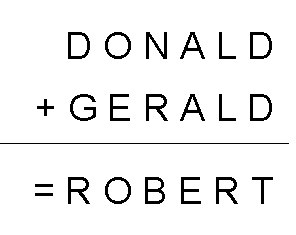
\includegraphics[scale=0.5]{litreview-example-alphametic}
\par\end{centering}
\caption{\label{fig:Alphametic-problem}Alphametic problem}
\end{figure}


Constraints are \emph{declarative} --- the statement of the problem
and the algorithms used to solve it are separated. This is an attractive
feature of constraints, since it can reduce the human effort required
to solve a problem. Various general purpose and specialized algorithms
exist for solving systems of constraints. A great variety of problems
can be expressed with constraints. The following list of subject areas
was taken from CSPLib \cite{csplib}:

\begin{itemize}
\item Scheduling (e.g. job shop scheduling \cite{martin-jobshop-96new}),
\item Design, configuration and diagnosis (e.g. template design \cite{proll-smith-templatedesign}),
\item Bin packing and partitioning (e.g. social golfer problem \cite{harvey01symmetry}),
\item Frequency assignment (e.g. the golomb ruler problem \cite{smith99golomb}),
\item Combinatorial mathematics (e.g. balanced incomplete block design \cite{frisch-symmetry-implied-04}),
\item Games and puzzles (e.g. maximum density still life \cite{smith-model-life}), 
\item Bioinformatics (e.g. discovering protein shapes \cite{protein-structure-problems}).
\end{itemize}

\section{Solving constraint problems}

The classical constraint satisfaction problem (CSP) has a finite set
of variables, each with a finite domain, and a set of constraints
over those variables. A solution to an instance of CSP is an assignment
to each variable, such that all constraints are simultaneously \emph{satisfied}
--- that is, they are all true under the assignment. Solvers typically
find one or all solutions, or prove there are no solutions. The decision
problem (`does there exist a solution?') is NP-complete \cite{apt-constraint-programming},
therefore there is no known polynomial-time procedure to find a solution.

The most common technique (and the one used by Minion) is to interleave
splitting (also called branching) and propagation. Splitting is the
basic operation of search, and propagation simplifies the CSP instance.
Apt views the solution process as the repeated transformation of the
CSP until a solution state is reached \cite{apt-constraint-programming}.
In this view, both splitting and propagation are transformations,
where propagation simplifies the CSP by removing values which cannot
take part in any solution. A splitting operation transforms a CSP
instance into two or more simpler CSP instances, and by recursive
application of splitting any CSP can be solved. 

Since splitting is an exponential-time solution method, it is important
that splitting is minimized by effective propagation. Much effort
has gone into developing propagation algorithms which are fast and
effective in removing values. Most propagation algorithms are specialized
to particular types of constraint (e.g. a vector of variables take
distinct values in any solution, the AllDifferent constraint). They
typically run in polynomial time.

Figure \ref{fig:solver-overview} is a simple representation of how
many constraint solvers (including Minion) work. The search element
is typically depth-first chronological backtracking by default, although
a solver will often allow different search algorithms to be programmed.
When searching, a variable and value must be selected. This can be
done statically or with a dynamic heuristic. The simplify component
contains a queue of constraints which need to be propagated. When
a constraint is propagated, and removes values from the variable domains,
the domain events cause other constraints to be added to the queue.
Propagation of constraints on the queue is iterated until the queue
is empty.

%
\begin{figure}
\begin{centering}
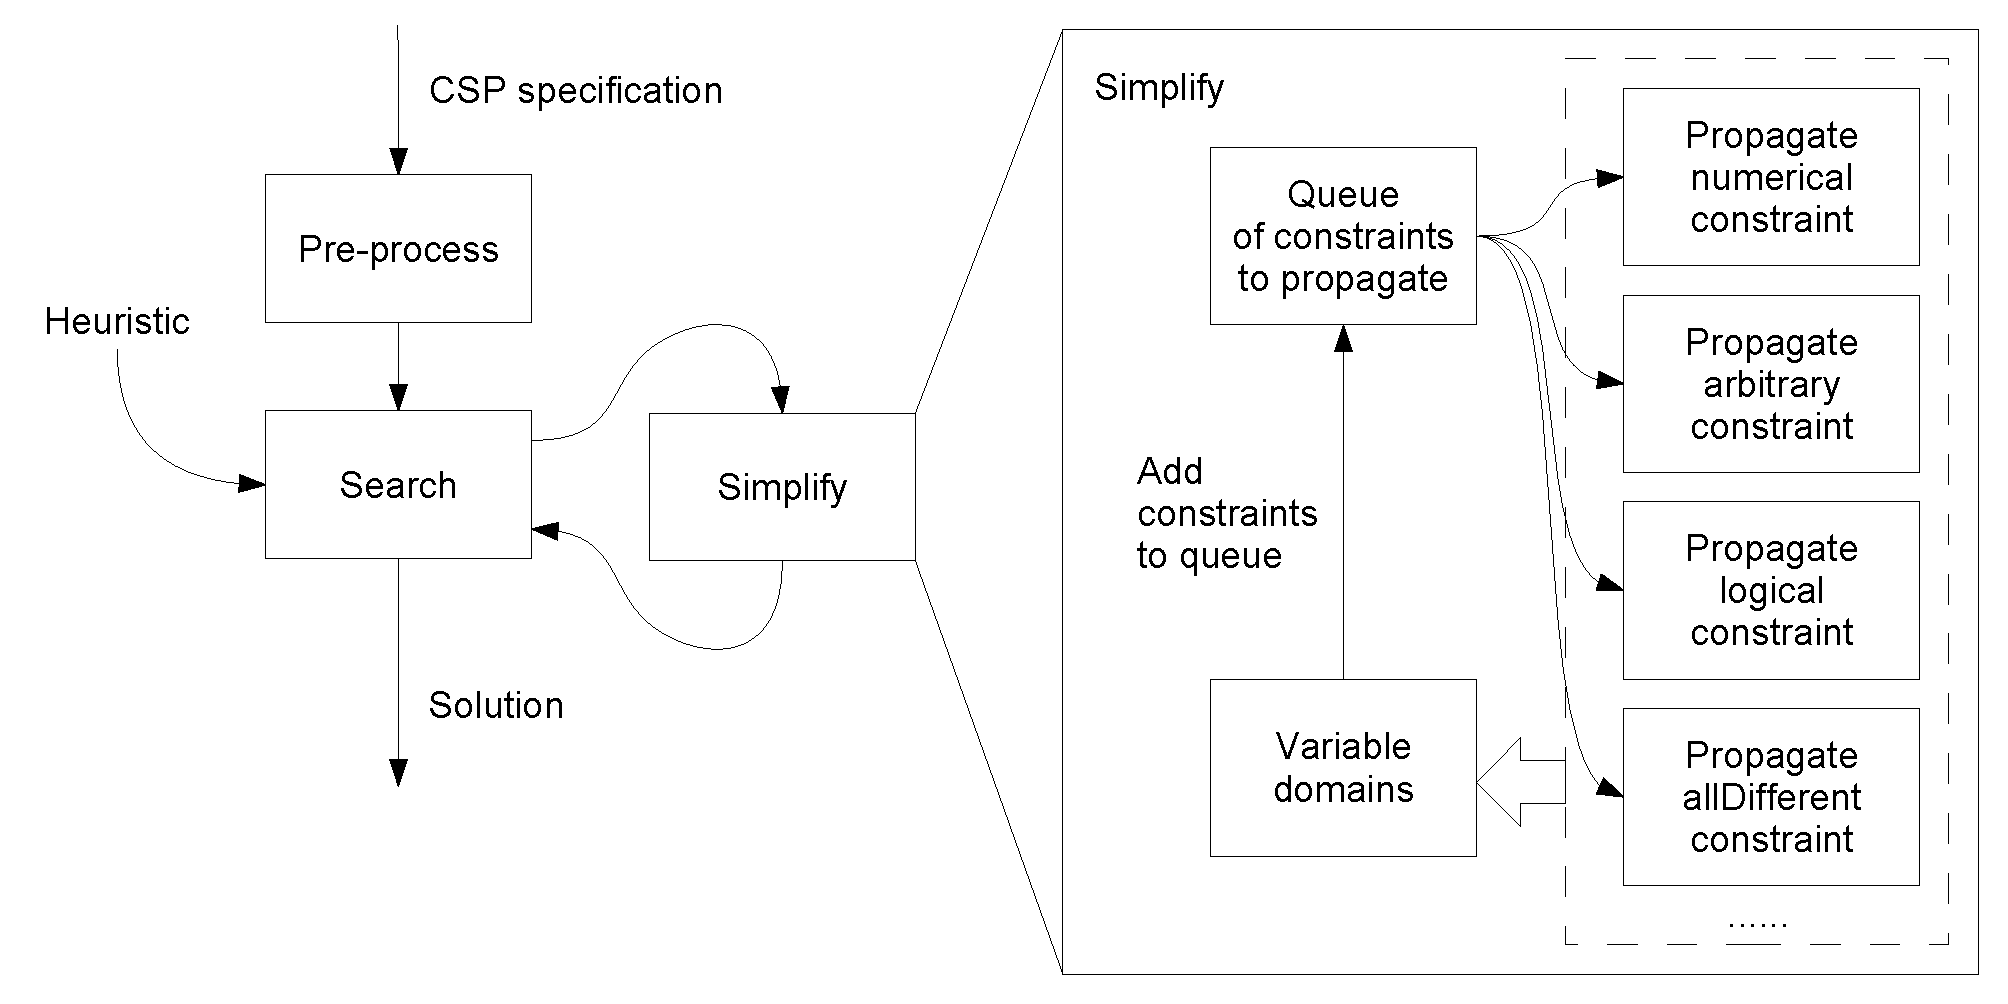
\includegraphics[width=1\textwidth]{litreview-solver-diagram}
\par\end{centering}

\caption{\label{fig:solver-overview}Overview of a constraint solver}

\end{figure}

\section{Minion}

Minion accepts a file describing an instance of CSP, and solves it
as described above. From the user's point of view, the most important
features are the set of constraints Minion can reason with, and the
types of variables which are supported. These are described later
in this document. This section deals with installing Minion and getting
started with it.


\subsection{Installing Minion}

The main Minion website is \url{http://minion.sourceforge.net/},
and this contains links to the download page. Currently, executables with and
without debug information are provided for Mac, Linux, Cygwin, and
Windows\footnote{The Windows binaries currently do not support compressed input
files.}.


\subsection{Installation instructions for Windows}

Download the Windows archive \texttt{minion-x.y.z-windows.tar.gz} and unpack,
you should find Minion executable \texttt{minion.exe}. The executable should
work from the Windows command shell \texttt{cmd.exe}. Minion requires the
Microsoft Visual C++ 2008 Redistributable Package\footnote{The Microsoft Visual C++
Redistributable Package can be downloaded from
\url{http://www.microsoft.com/downloads/details.aspx?FamilyID=a5c84275-3b97-4ab7-a40d-3802b2af5fc2&displaylang=en}.}
to work. Please note that the package for Visual C++ 2010 will \emph{not} work.

Alternatively, you can get the archive \texttt{minion-x.y.z-cygwin.tar.gz} which
also contains some additional required DLL files.


\subsection{Installation instructions for Mac}

Download the Mac archive \texttt{minion-x.y.z-mac.tar.gz} and unpack. The contents
include universal binary \texttt{minion} which should work on both Intel and PowerPC
Macs with Mac OS X 10.4.2 or later.


\subsection{Installation instructions for Linux-x86 or x64}

Download the Linux archive \texttt{minion-x.y.z-linux.tar.gz} and unpack. It contains
the binary \texttt{minion}. The executable is linked statically.

\bigskip

All versions come with a debug variant as well. The debug executables are
contained in the \texttt{minion-x.y.z-debug-<os>.tar.gz}.


\subsection{Compilation instructions}

If there is no executable which works on your computer, you can use
the source package (named \texttt{minion-x.y.z-source.tar.gz}).

Minion uses the CMake\footnote{\url{http://www.cmake.org}} build system to check
for the required and optional components. Without any additional flags, the
standard binary will be built. The earliest version of CMake the build was
tested with is 2.4.7.

Note that you need at least g++ version 3.4.2 to compile Minion. Furthermore
boost\footnote{\url{http://www.boost.org/}} is required to build Minion. Any
version between 1.33 and 1.42.0 inclusive should work. If you have installed
boost in a non-standard location or CMake does not find it for some other
reason, you can try setting the environment variable \verb+BOOST_ROOT+ to your
boost installation directory for CMake 2.6, or \verb+Boost_INCLUDE_DIR+ to the
location of the boost header files for CMake 2.4.

The g++ distributed with Cygwin does \emph{not} compile Minion correctly because
of differences in exception handling in Unix and Windows. You have to compile
your own version of g++ and use this to compile Minion.

To compile, create a new directory for the build, and issue the
following commands on Unix:

\begin{verbatim}
cmake <path/to/minion>
make minion
\end{verbatim}

where \verb+<path/to/minion>+ is the path to the Minion distribution (the
directory which contains \verb+CMakeLists.txt+). The Cygwin version of CMake
seems to have a bug; run it twice to get Minion to compile and link correctly.

On Windows, use CMake to generate Visual Studio project files. You can then open
the project file in Visual Studio and compile it. The build was tested with Visual
Studio 9 2008.

If you have at least 2GB of RAM and a dual-core processor, you may prefer to
use
\begin{verbatim}
make minion -j2
\end{verbatim}
instead. As a rule of thumb, you should have 1GB of RAM for every compile
process. To build minion-debug, run
\begin{verbatim}
cmake -DDEBUG=1 <path/to/minion>
\end{verbatim}
instead of
\begin{verbatim}
cmake <path/to/minion>
\end{verbatim}
CMake caches the configuration between runs. If you built the debug binary first
and then want to build the non-debug version, you have to explicitely disable
that option, i.e.\ run
\begin{verbatim}
cmake -DDEBUG=0 <path/to/minion>
\end{verbatim}

More details on compile-time options can be found in section~\ref{compiletime}.

\subsection{Trying out the executable}

On all platforms, Minion needs to be run from a command shell so that
the output can be seen. If you go to the Minion directory in a shell
and run the executable, it should output version information and a
help message. 


\subsection{The debug variant}

One would normally use the non-debug variant of minion, which runs
at full speed. However, if some unexpected behaviour is observed,
running the debug variant may be helpful. It contains a large number
of assertions and other checks, and may bring to light a problem with
the input or an internal bug.

The CMake constants you should set to \verb+1+ to get a binary suitable for
debugging are \verb+DEBUG+ and \verb+INFO+.


\subsection{Minion online help}

To see the root page of the help system, run Minion with \texttt{help}
as the only argument. The help system is hierarchical, with the following
top-level categories: constraints, input, switches and variables,
with contents as follows:

\begin{description}
\item [{\texttt{constraints}}] This category contains a description of
every constraint which is allowed in the input CSP.
\item [{\texttt{input}}] Information about the input file format.
\item [{\texttt{switches}}] Information about command-line switches.
\item [{\texttt{variables}}] A description of each type of CSP variable
supported in Minion.
\end{description}
To access the help for the alldiff constraint, for example, the command
would be \texttt{minion help constraints alldiff}. The full documentation
provided by the Minion executable is reproduced in the Appendix of 
this manual.


\subsection{Basic Minion use}

As a simple example of Minion input, we modelled the alphametic puzzle
in figure \ref{fig:Alphametic-problem}. The Minion input file shown
below consists of two sections: the variables, in which the 10 CSP
variables are declared along with their initial domains; and the constraints.
The allDifferent constraint in the example above is mapped into gacalldiff
here. The numerical constraint is translated into two constraints
as follows: $x+y=z$ is mapped to $x+y-z\le0$ and $x+y-z\ge0$ and
these two are represented using weightedsumleq and weightedsumgeq
respectively. The coefficients are specified first, with the coefficients
of ROBERT negated, followed by the list of variables.

\begin{verbatim}
MINION 3

**VARIABLES**

DISCRETE a {0..9}
DISCRETE b {0..9}
DISCRETE d {0..9}
DISCRETE e {0..9}
DISCRETE g {0..9}
DISCRETE l {0..9}
DISCRETE n {0..9}
DISCRETE o {0..9}
DISCRETE r {0..9}
DISCRETE t {0..9}

**CONSTRAINTS**

gacalldiff([a,b,d,e,g,l,n,o,r,t])

weightedsumleq([100000,10000,1000,100,10,1,
100000,10000,1000,100,10,1,
-100000,-10000,-1000,-100,-10,-1],
[d,o,n,a,l,d,g,e,r,a,l,d,r,o,b,e,r,t],0)

weightedsumgeq([100000,10000,1000,100,10,1,
100000,10000,1000,100,10,1,
-100000,-10000,-1000,-100,-10,-1],
[d,o,n,a,l,d,g,e,r,a,l,d,r,o,b,e,r,t],0)

**EOF**
\end{verbatim}

This example is in the Minion distribution, in directory benchmarks/small.
Executing \texttt{minion benchmarks/small/donaldgeraldrobert.minion}
gives the solution $A=4, B=3, D=5, E=9, G=1,
L=8, N=6, O=2, R=7, T=0.$

\chapter{Minion Internals}

This chapter explains several details about Minion's internals, which are useful to know when trying to get the most from Minion.

\section{Variable Types}

Minion's input language is purposefully designed to map exactly to Minion's internals. Unlike most other constraint solvers, Minion does not internally add extra variables and decompose large complex constraints into small parts. This provides complete control over how problems are implemented inside Minion, but also requires understanding how Minion works to get the best results.

For those who, quite reasonably, do not wish to get involved in such details, 'Tailor' abstracts away from these details, and also internally implements a number of optimisations.

One of the most immediately confusing features of Minion are the variable types. Rather than try to provide a "one-size-fits-all" variable implementation, Minion provides four different ones; \BOOL, \DISCRETE, \BOUND and \SPARSEBOUND.  First we shall provide a brief discussion of both what these variables are, and a brief discussion of how they are implemented currently.

\begin{description}
\item[\BOOL] Variables with domain \(\{0,1\}\). Uses special optimised data structure.
\item[\DISCRETE] Variables whose domain is a range of integers. Memory usage and the worst-case performance of most operations is O(domain size). Allows any subset of the domain to be represented.
\item[\BOUND] Variable whose domain is a range of integers. Memory usage and the worst-case performance of all operations is O(1). During search, the domain can only be reduced by changing one of the bounds.
\item[\SPARSEBOUND] Variable whose domain is an arbitary range of integers. Otherwise identical to BOUND.
\end{description}

It appears one obvious variable implementation, \texttt{SPARSEDISCRETE}, is missing. This did exist in some very early versions of Minion but due to bugs and lack of use was removed. 

Some of the differences between the variable types only effect performance, whereas some others can effect search size. We provide these here.

\begin{enumerate}
\item In any problem, changing a \BOOL variable to a \DISCRETE, \BOUND or \SPARSEBOUND variable with domain \(\{0,1\}\) should not change the size of the resulting search. \BOOL should always be fastest, followed by \DISCRETE, \BOUND and \SPARSEBOUND.

\item A \BOUND variable will in general produce a search with more nodes per second, but more nodes overall, than a \DISCRETE variable.

\item Using \SPARSEBOUND or \BOUND variables with a unary constraint imposing the sparse domain should produce identical searches, except the \SPARSEBOUND will be faster if the domain is sparse. 
\end{enumerate}

As a basic rule of thumb, Always use \BOOL for Boolean domains, \DISCRETE for domains of size up to around 100, and the \BOUND. With \DISCRETE domains, use the \texttt{w-inset} constraint to limit the domain. When to use \SPARSEBOUND over \BOUND is harder, but usually the choice is clear, as either the domain will be a range, or a set like \(\{1,10,100,100\}\).

\section{Choosing Between Minion's Constraints}

Minion has many constraints which at first glance appear to do almost identical things. These each have trade-offs, some of which are difficult to guess in advance. This section will provide some basic guidance.

One of the major design decisions of Minion's input language is that it provides in the input language exactly what it provides internally. Unlike most other constraint solvers, Minion does not break up constraints into smaller pieces, introduce new variables or simplify or manipulate constraints. This provides complete control over how Minion represents your problem, but also leads to a number of annoyances.

Probably the first thing you will notice it that Minion has neither a ``sum equals'' or ``weighted sum equals'' constraint. This is because the most efficiently we could implement such a constraint was simply by gluing together the sumleq and the sumgeq constraints. Minion could provide a wrapper which generated the two constraints internally, but this would go against the transparency. Of course if in the future a more efficient implementation of sumeq was found, it may be added.

The \texttt{watchsumgeq} and \texttt{watchsumleq} are varients on the algorithm used to implement SAT constraints. They are faster than \texttt{sumleq} and \texttt{sumgeq}, but only work when summing a list of Booleans to a constant. Further \texttt{watchsumgeq} performs best when the value being summed to is small, and \texttt{watchsumleq} works best when the value being summed to is close to the size of the input vector.

Minion does not attempt to simplify constraints, so constraints such as \texttt{sumgeq([a,a,a], 3)} are not simplified to \texttt{sumgeq([a],1)}. This kind of simplification, done by hand, will often improve models. Further, and importantly in practice, Minion pre-allocates memory based on the initial domain size of variables. If these are excessively slack, this can hurt performance throughout search.

Some constraints in Minion do not work on \texttt{BOUND} and \texttt{SPARSEBOUND} variables, in particular \texttt{gacalldiff} and \texttt{watchelement}. These two constraints are in general better when they can be used.

\section{Compile-time options}\label{compiletime}

There are a number of flags which can be given to Minion at compile time to
affect the resulting executable. These flags are prone to regular changes. By
searching the Minion source code, you may find others. These undocumented ones
are prone to breakage without warning.

The following flags are considered "blessed", and are fully tested (although in
future versions they may be removed or altered). Adding any of these flags
will probably slow the resulting Minion executable.

All of these flags have to be passed to \texttt{cmake} with the \verb+-D+
switch; for example
\begin{verbatim}
cmake -DNAME=MyMinion <path/to/minion>
\end{verbatim}
Again, keep in mind that \texttt{cmake} caches its configuration -- if you run
it again without specifying \verb+NAME+, it will assume the name you have given
before and \emph{not} the default.

\begin{description}
\item[\texttt{NAME=name}] Overrides Minion's default and names the executable
\verb+name+.
\item[\texttt{DEBUG=1}] Turns on a large number of internal consistency checks in
minion. This executable is much slower than normal minion, but vital when trying
to debug problems.
\item[\texttt{SLOW\_DEBUG=1}] Turns on even more internal checking; the resulting
executable will be much slower than standard Minion.
\item[\texttt{PRINT=1}] (Only meaningful with \texttt{DEBUG=1}) Turns on
more printing of information.
\item[\texttt{QUICK=1}] For optimisation reasons, Minion usually compiles many copies of
every constraint. This flag makes Minion compile each constraint only once. This
drastically reduces the time to compile and the size of the executable, but the
resulting executable is slower. This should never effect the results Minion
produces.
\item[\texttt{INFO=1}] Makes minion output a large, but poorly documented, set of
information about how search is progressing. This flag is useful for debugging
but should not be used for trying to following search (use the command line flag
-dumptree instead). This option is likely to be replaced with a more useful dump
of search in a future version of Minion.
\item[\texttt{UNOPTIMISED=1}] Turn off all compiler optimisation, so Minion can be
usefully checked in gdb.
\item[\texttt{PROFILE=1}] Set compiler optimisation flags that allow Minion to be
better profiled. Implies \texttt{UNOPTIMISED=1}.
\item[\texttt{GPROF=1}] (Only meaningful with \texttt{PROFILE=1}) Set compiler flags to profile the binary with
\texttt{gprof}.
\item[\texttt{REENTER=1}] Compile Minion so it is reenterent (more than one
problem can exist in memory at a time). At present reenterence is not used for
anything, and will only slightly slow Minion.
\item[\texttt{THREADSAFE=1}] Compile thread-safe Minion. Does not have any effect
right now.
\item[\texttt{SMALL=1}] Build a small binary by passing \verb+-Os+ to the
compiler.
\item[\texttt{WDEG=1}] Enable weighted degree variable heuristic. This may or may
not speed up Minion.
\item[\texttt{WTRIG=1}] Enable a weighted queue of triggers which will process the
cheapest trigger first. This only affects triggers of the same type. This may or
may not speed up Minion.
\item[\texttt{BACK\_VEC=1}] Keep backtrack memory in a vector instead of a
continuous block of memory.
\item[\texttt{CACHE\_MALLOC=1}] (Only meaningful with \texttt{BACK\_VEC=1}) Enable
caching malloc.
\item[\texttt{DISTCC=1}] Use \verb+distcc+ (if found). Experimental.
\end{description}

Furthermore the environment variable \verb+$CPU+ is taken into account when
running \texttt{cmake}. The contents of this variable are passed on to the
compiler without any processing; usually one would want to use it as a means of
specifying machine-specific compiler flags, such as producing code for a
specific CPU.

\subsection{Required and optional components}

Boost is required to build Minion (at least version 1.33). Bzip2 and Zlib are
optional, if they are not present, you will not be able to read compressed input
files. If a Common Lisp binary (\texttt{clisp}) is found, you will be able to
build the LISP generators. If you have a \texttt{doxygen} executable, you will
be able to generate the API documentation. If you have a \texttt{pdflatex}
executable and a UNIX-like system, you will be able to generate the PDF
documentation.

\subsection{Selective compilation of constraints}

The most time-consuming part of the Minion compilation process is the
compilation of all the constraints. If not all constraints are required, the
user may specify the constraints to be compiled into the binary in two ways.

When running \texttt{cmake} one can give it the \verb+-DCONSTRAINTS="<list>"+
flag to specify the semicolon-separated list of constraints to be compiled,
e.g.\
\begin{verbatim}
cmake -DCONSTRAINTS="sumleq;sumgeq" <path/to/minion>
\end{verbatim}

Alternatively, one can specify the name of a Minion input file or a file
containing a list of constraints with the \verb+-DCONSTRAINTS_FILE=<file>+
option, e.g.\
\begin{verbatim}
cmake -DCONSTRAINTS_FILE=input.minion <path/to/minion>
\end{verbatim}
Note that this does not work with compressed input files.

\chapter{Minion in Practice}
The previous chapter clearly outlined what the constructs of a Minon file are, including what the variable types are and which type of constraint should be used when. This chapter takes a more practical role, outlined within are 7 minion example files which are clearly commented so that the user can see what a minion file looks like in practice. Comments in minion start with a $\sharp$, however for reasons of ease of reading all lines of actual code be it Minion or Essence' are shown in typewriter text and comments are inserted in normal text. The first file is a modified version of the one that all the minion developers turn to when modelling a new problem in minion. It shows exactly what a minion file can include and what the syntax is for all the possible sections. If you are modelling a problem as minion than we recommend you take a copy of this file and edit it appropriately, as this will help to guide you through the modelling process. The rest of this chapter contains versions  of the minion input examples introduced in the Tailor chapter of this manual. These are all produced automatically by tailor from the Essence' specification given in that chapter. We hope the comments will clarify exactly what these files mean. These examples can be used as the bases to implement any similar problems. The Minion overview is completed in the last chapter where a full list of all the constraints is given, including a brief overview of how each operates. 

\section{Minion Example File}
This file does not really relate to any English problem description, although it does parse and run,  it is an example which clearly shows all of the possible Minion input file constructs. If you are modelling a problem as minion than we recommend you take a copy of this file and edit it appropriately, as this will help to guide you through the modelling process. It can be found in the \begin{verbatim}summer_school\end{verbatim} directory and is called \begin{verbatim}format_example.minion\end{verbatim} we have added comments  to explain the different sections to the novice user. 

\begin{verbatim}
MINION 3
\end{verbatim}

This file includes an example of all the different inputs  you can give to Minion.  It is a very good place to start from when modelling  problem in the Minion specification. 

 The first section is where all the variables are declared.
 \begin{verbatim}
**VARIABLES**
\end{verbatim}

There are 4 type of variables. Booleans don't need a domain and are formated as follows:
 \begin{verbatim}
BOOL bo    
 \end{verbatim}

Internally, Bound variables are stored only as a lower  and upper bound whereas discrete variables allow any sub-domain.
Bound variables need a domain given as a range as follows: 
 \begin{verbatim}
BOUND b {1..3}   
 \end{verbatim}

Discrete vars also need a domain given as a range as follows:   
\begin{verbatim}
DISCRETE d {1..3} 
\end{verbatim}

Sparse bound variables take a sorted list of values as follows:
\begin{verbatim}
SPARSEBOUND s {1,3,6,7} 
\end{verbatim}

We can also declare matrices of variables. The first example is a matrix with 3 variables: q[0],q[1] and q[2].
\begin{verbatim}
DISCRETE q[3] {0..5} 
\end{verbatim}

The second example is of a 2d matrix, where the variables are bm[0,0], bm[0,1], bm[1,0], bm[1,1].
\begin{verbatim}
BOOL bm[2,2] 
\end{verbatim}

The third example shows how to declare a matrix with more indices. You can have as many indices as you like!
\begin{verbatim}
BOOL bn[2,2,2,2] 
\end{verbatim}

In this next section, which is optional, you can define tuplelists. Tuplelists provide a method of defining sets of tuples which can then be used in \texttt{table} and \texttt{negativetable} constraints. Defining these in a \texttt{**TUPLELIST**} does not change the search, but can save memory by reusing the same list of tuples in multiple constraints.The input is: $\langle$name$\rangle$ $\langle$num$\_$of$\_$tuples$\rangle$ $\langle$tuple$\_$length$\rangle$ $\langle$numbers$\ldots \rangle$.
\begin{verbatim}
**TUPLELIST**
Fred 3 3
0 2 3
2 0 3
3 1 3
\end{verbatim}

The next thing to declare are the constraints which go in  this section.
\begin{verbatim}
**CONSTRAINTS**
\end{verbatim}

Constraints are defined in the same way as functions are in most programming paradigms!  A complete list of constraints can be found at the end of  the manual. The two following constraints very simply set bo=0 and b=d.
\begin{verbatim}
eq(bo, 0)
eq(b,d)
\end{verbatim}

Note that except in special cases (the \texttt{reify} and \texttt{reifyimply} constraints), Minion constraints cannot be nested. For example \texttt{eq(eq(bo,0), d)} is not valid. Such constraints must be written by manually adding extra variables.

To get a single variable from a matrix, you index it with square brackets using commas to delimitate the dimensions of the matrix. The first example following is a 1D matrix, the second in 4D. 
\begin{verbatim}
eq(q[1],0)
eq(bn[0,1,1,1], bm[1,1])
\end{verbatim}

It's easy to get a row or column from a matrix.  You use $\_$ in the indices you want to vary.  Giving a matrix without an index simply gives all the variables in that matrix. The following shows how flattening occurs...\\
$[bm] == [ bm[\_,\_] ] == [ bm[0,0], bm[0,1], bm[1,0], bm[1,1] ]$\\
$[ bm[\_,1] ] = [ bm[0,1], bm[1,1] ]$\\
$[ bn[1,\_,0,\_] = [ bn[1,0,0,0], b[1,0,0,1], b[1,1,0,0], b[1,1,0,1] ]$\\

You can string together a list of such expressions as in the following example:
\begin{verbatim}
lexleq( [bn[1,_,0,_], bo, q[0]] , [b, bm, d] )
\end{verbatim}

So the parser can recognise them you must always put [ ] around any matrix expression, so lexleq(bm, bm) is invalid, but the following is valid:
\begin{verbatim}
lexleq( [bm], [bm] )
\end{verbatim}

An example of a constraint which uses tuples
\begin{verbatim}
table([q], Fred)
\end{verbatim}

You do not have to pre-declare tuples, you can write them explicitly if you wish. The above constraint for example is equivalent to:
\begin{verbatim}
table([q],{ <0,2,3>,<2,0,3>,<3,1,3> })
\end{verbatim}

The last section is the search section. This section is optional, and allows some limited control over the way minion searches for a solution. Note that everything in this section can be given at most once.
\begin{verbatim}
**SEARCH** 
\end{verbatim}

You give the variable ordering by listing each of the variables in the order you wish them to be searched. You can either list each of the variables in a matrix individually by giving the index of each variable, or you can just state the matrix in which case it goes through each of the variables in turn. If you miss any of the variables out than these variables are not branched on. Note that this can lead to Minion reporting invalid solutions, so use with care! If you don't give an explicit variable ordering, than one is generated based on the order the variables are declared. If you give a \texttt{-varorder} on the command line, that will only consider the variable given in the \texttt{VARORDER}.
\begin{verbatim}
VARORDER [bo,b,d,q[_]] 
\end{verbatim}

You give the value order for each variable as either \texttt{a} for ascending or \texttt{d} for descending. The value orderings are given in the same order as the variable ordering. For example, to make the variable b by searched in descending order you make the second term into a \texttt{d} as the above variable ordering shows it to be the second variable to be searched. The default variable order is ascending order for all variables.
\begin{verbatim}
VALORDER [a,a,d,a]
\end{verbatim}

You can have one objective function which can be either to maximise or minimise any single variable. To minimise a constraint, you should assign it equal to a new variable.
\begin{verbatim}
MAXIMISING bo
# MINIMISING x3
\end{verbatim}

The print statement takes a 2D matrix of things to print. The following example prints both the variables bo and q, putting these in double square brackets turns them into a 2D matrix so they are acceptable input.  You can also give:  PRINT ALL (the default) which prints all variables and PRINT NONE which turns printing off completely.
\begin{verbatim}
PRINT [ [bo, q] ]
\end{verbatim}


The file must end with the **EOF** marker! Any text under that is ignored, so you can write 
whatever you like (or nothing at all...)
\begin{verbatim}
**EOF**
\end{verbatim}

The only remaining part of Minion's input language are its many constraints. These are listed in the Appendix.

\section{The Farmers Problem}
The Farmers Problem is a very simple problem which makes a very good example to be the first CP that you model. The problem is as follows:  A farmer has 7 animals on his farm: pigs and hens. They all together have 22 legs. How many pigs (4 legs) and how many hens(2 legs) does the farmer have? These files can be found in \texttt{/summer\_school/examples}. The Essence' file is named \texttt{FarmersProblem.eprime} and the Minion file is \texttt{FarmersProblem.minion}

The Essence' specification of this (which was explained in detail in the Tailor section is as follows:

\begin{verbatim}
find pigs, hens: int(0..7)

such that

pigs + hens = 7,
pigs * 4 + hens * 2 = 22
\end{verbatim}

The Minion input file for this is:
\begin{verbatim}
MINION 3

\end{verbatim}
There are two variables pigs and hens  both have domain {0..7}

\begin{verbatim}
**VARIABLES**
DISCRETE pigs {0..7}
DISCRETE hens {0..7}
\end{verbatim}

Both variables pigs and hens should be printed and the variable ordering is search pigs than hens.
\begin{verbatim}
**SEARCH**

PRINT [[pigs],[hens]]

VARORDER [pigs,hens]


**CONSTRAINTS**
\end{verbatim}

The following two constraints relate to the following $(pigs \times 4) + (hens \times 2) = 22$. There is no weighted sum constraint in Minion so you should use the weighted sum less than and equal to constraint and the weighted sum greater than and equal to constraint. You read this as  $(hens \times 2) + (pigs \times 4)) \leq 22$ and $(hens \times 2) + (pigs \times 4)  \geq 22$.
\begin{verbatim}
weightedsumgeq([2,4], [hens,pigs], 22)
weightedsumleq([2,4], [hens,pigs], 22)
\end{verbatim}

The following two constraints relate to the following $pigs + hens = 7$. There is no sum constraint in Minion so you should use the sum less than and equal to constraint and the sum greater than and equal to constraint. You read this as $hens + pigs \leq 7$ and $hens + pigs \geq 7$.
\begin{verbatim}
sumleq([hens,pigs], 7)
sumgeq([hens,pigs], 7)
**EOF**
\end{verbatim}

\section{Cryptarithmetic}
The second problem outlined is a very famous Cryptarithmetic puzzle: SEND + MORE = MONEY. These files can be found in \texttt{/summer\_school/examples} the Essence' file is \texttt{SENDMOREMONEY.eprime} and the Minion file is \texttt{SENDMOREMONEY.minion}. The Essence' specification is as follows:

\begin{verbatim}
find S,E,N,D,M,O,R,Y : int(0..9)

such that

1000*S + 100*E + 10*N + D + 
1000*M + 100*O + 10*R + E =
10000*M + 1000*O + 100*N + 10*E + Y,

alldiff([S,E,N,D,M,O,R,Y])
\end{verbatim}

The Minion model is then:

\begin{verbatim}
MINION 3
\end{verbatim}

There are 8 variables: S,E,N,D,M,O,R,Y all with domains 0 to 9.
\begin{verbatim}
**VARIABLES**
DISCRETE S {0..9}
DISCRETE E {0..9}
DISCRETE N {0..9}
DISCRETE D {0..9}
DISCRETE M {0..9}
DISCRETE O {0..9}
DISCRETE R {0..9}
DISCRETE Y {0..9}
\end{verbatim}

Search the variables in the order S, E, N, D, M, O, R, Y and print the same variable in this order.
\begin{verbatim}
**SEARCH**

PRINT [[S],[E],[N],[D],[M],[O],[R],[Y]]

VARORDER [S,E,N,D,M,O,R,Y]
\end{verbatim}

The first constraint is an all different which is across all variables this is an implicit constraint in the problem, as all the letters represent different numbers.
\begin{verbatim}
**CONSTRAINTS**

alldiff([ S, E, N, D, M, O, R, Y])
\end{verbatim}

The second constraint represents:$(1000 \times S) + (100 \times E) + (10 \times N) + D +  (1000 \times M) + (100 \times O )+ (10 \times R) + E = (10000 \times M) + (1000 \times O) + (100 \times N) + (10 \times E) + Y$.  The first thing the model does is rewrite this expression to make it equal to a number, in this case 0. So this expression becomes: $(10000 \times M) + (1000 \times O) + (100 \times N) + (10 \times E) + Y - (1000 \times S)  - (100 \times E) - (10 \times N) - D - (1000 \times M) - (100 \times O) - (10 \times R) - E = 0$. The terms are then rearranged so the same weights are together and the positive numbers are first this then becomes: $Y + (10 \times E) + (100 \times N) + (1000 \times O) + (10000 \times M) -D - E - (10 \times N) - (10 \times R) - (100 \times E) - (100 \times O)  - (1000 \times M) - (1000 \times S) = 0$. Minion does not have a weighted sum equals constraint, so this is represented as one weighted sum less than or equal to and one weighted sum greater than or equal to. The two constraints are then: $Y + (10 \times E) + (100 \times N) + (1000 \times O) + (10000 \times M) -D - E - (10 \times N) - (10 \times R) - (100 \times E) - (100 \times O)  - (1000 \times M) - (1000 \times S) \leq 0$ and $Y + (10 \times E) + (100 \times N) + (1000 \times O) + (10000 \times M) -D - E - (10 \times N) - (10 \times R) - (100 \times E) - (100 \times O)  - (1000 \times M) - (1000 \times S) \geq 0$.

\begin{verbatim}
weightedsumgeq(
	[1,10,100,1000,10000,-1,-1,-10,-10,-100,-100,-1000,-1000], 
	[Y,E,N,O,M,D,E,N,R,E,O,M,S], 0)
weightedsumleq(
	[1,10,100,1000,10000,-1,-1,-10,-10,-100,-100,-1000,-1000],
	[Y,E,N,O,M,D,E,N,R,E,O,M,S], 0)

**EOF**
\end{verbatim}

\section{The Eight Number Puzzle}
The eight number puzzle asks you to label the nodes of the graph shown in Figure~\ref{fig:8puzzle} with the values 1 to 8 such that no two connected nodes have consecutive values.  These files can be found in /summer\_school/examples the Essence' file is EightPuzzleDiagram.eprime and the Minion file is EightPuzzleDiagram.minion. The Essence' specification is as follows:

\begin{figure}[htp]
\centering
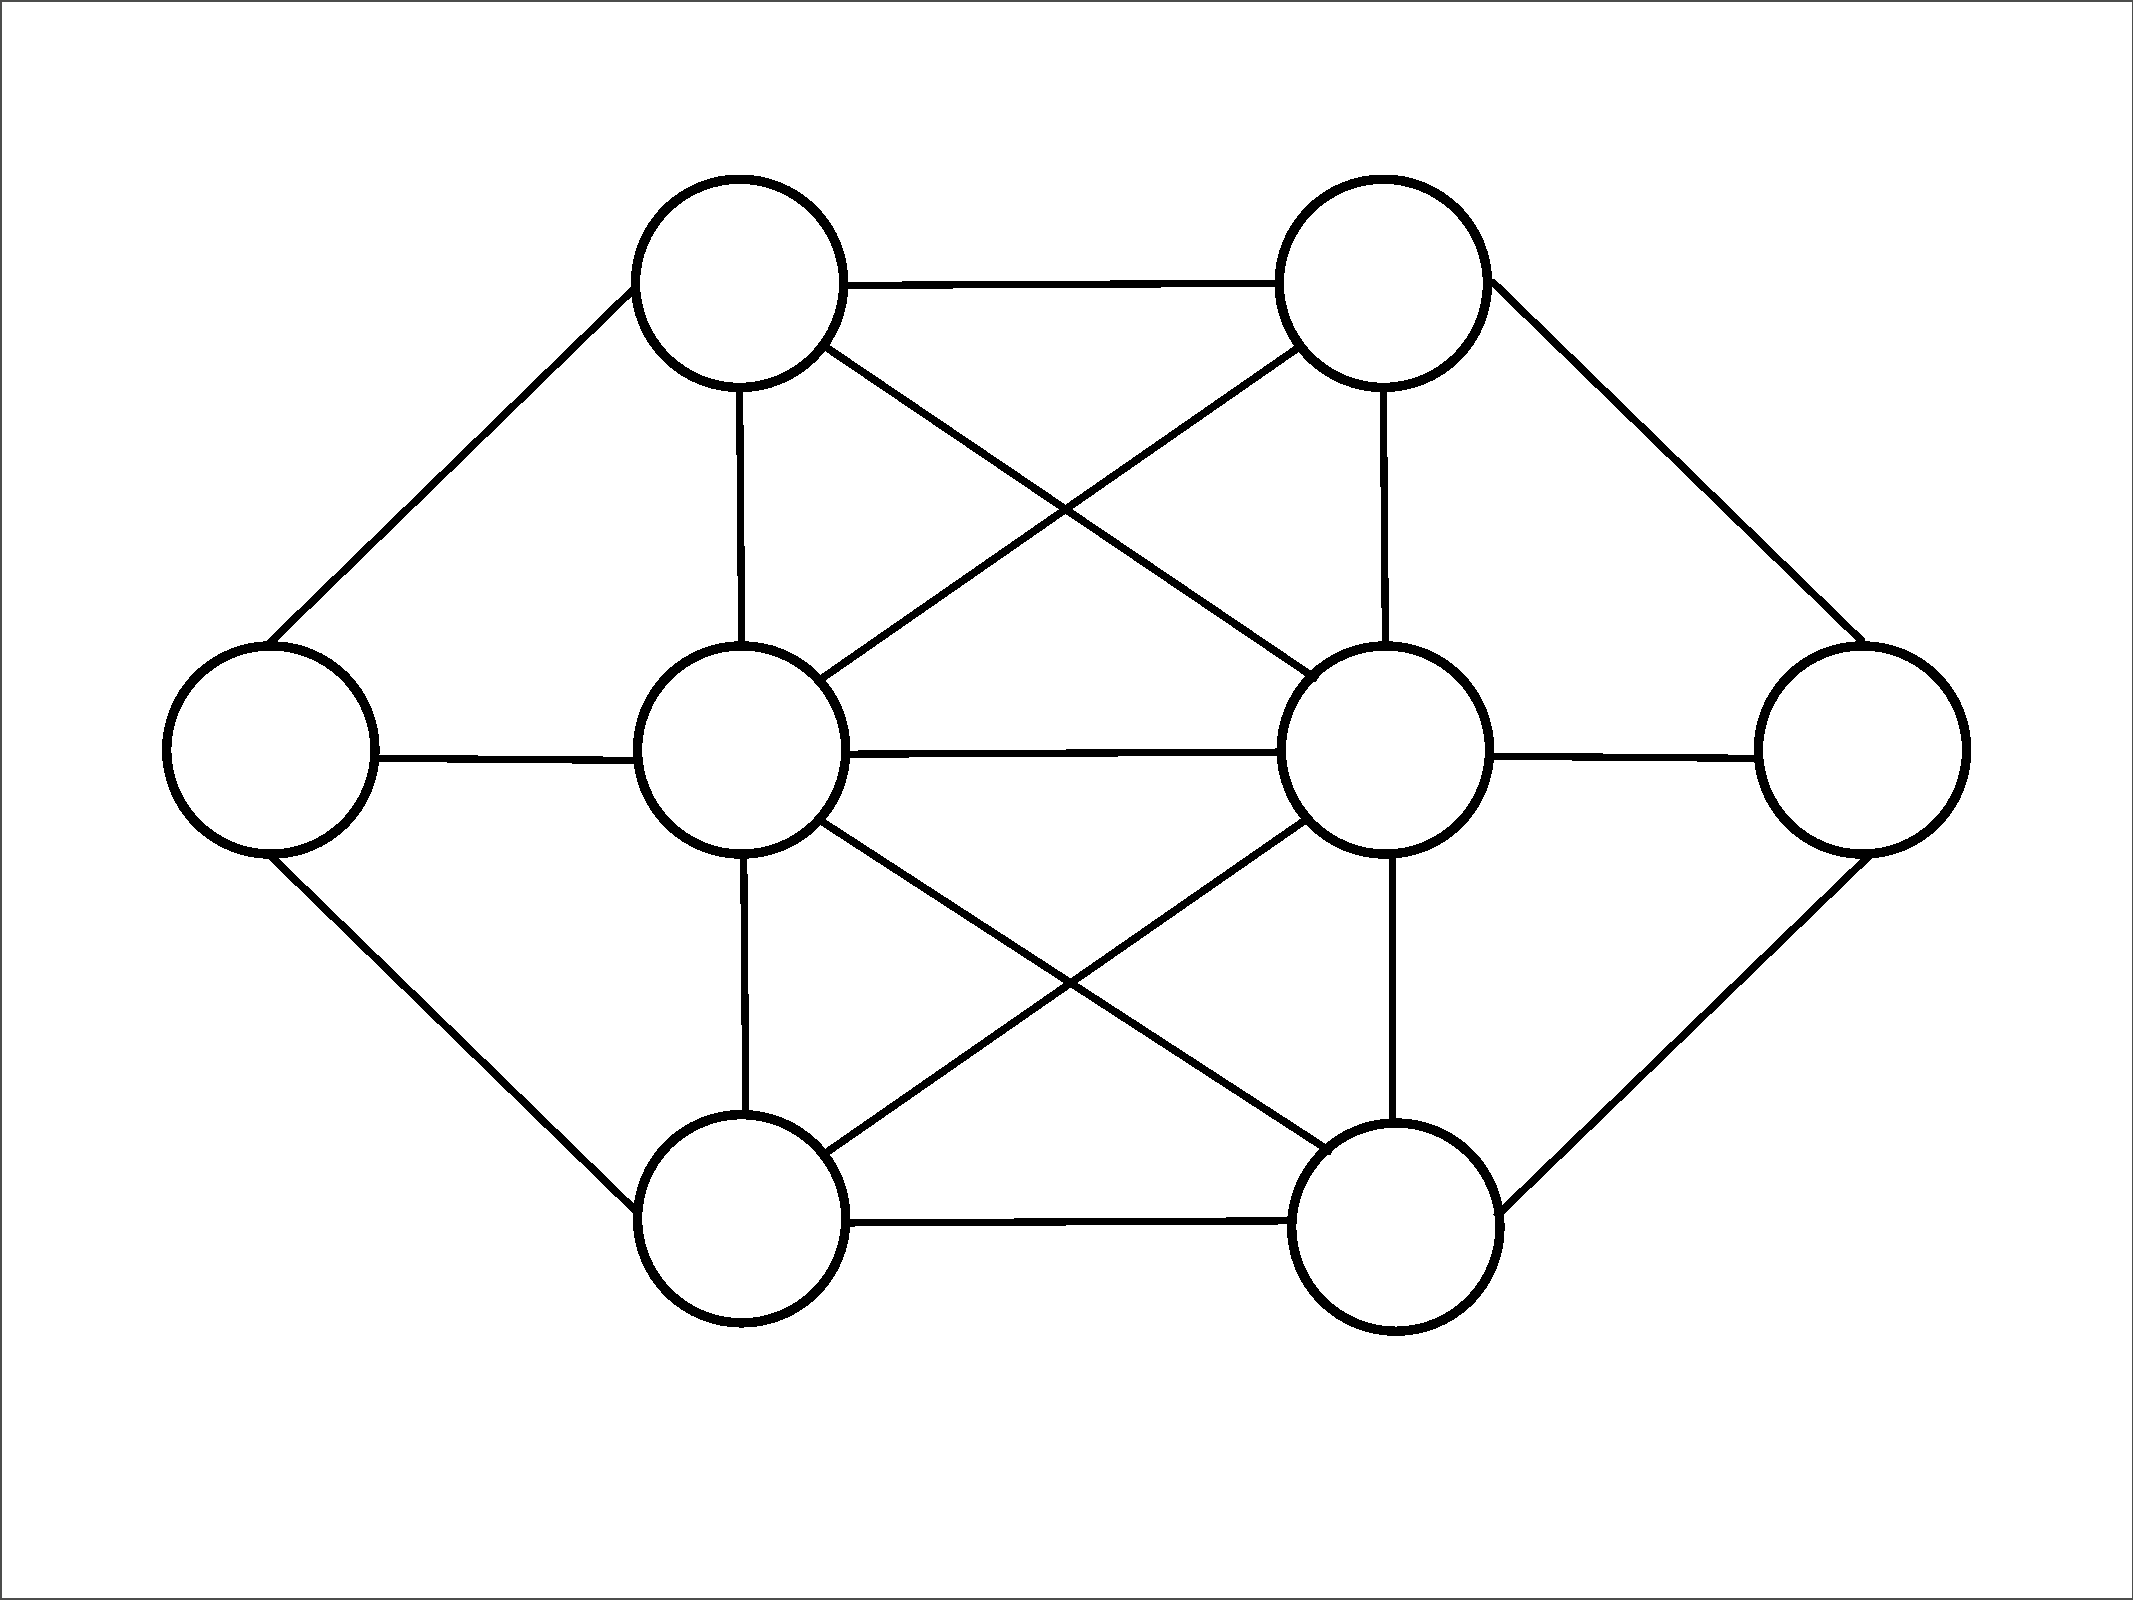
\includegraphics[scale=0.25] {EightPuzzleDiagram.pdf} 
\caption{Graph which represents The Eight Number Puzzle}
\label{fig:8puzzle}
\end{figure}

\begin{verbatim}
find circles: matrix indexed by [int(1..8)] of int(1..8)

such that

alldiff(circles),
| circles[1] - circles[2] | > 1,
| circles[1] - circles[3] | > 1,
| circles[1] - circles[4] | > 1,
| circles[2] - circles[3] | > 1,
| circles[3] - circles[4] | > 1,
| circles[2] - circles[5] | > 1,
| circles[2] - circles[6] | > 1,
| circles[3] - circles[5] | > 1,
| circles[3] - circles[6] | > 1,
| circles[3] - circles[7] | > 1,
| circles[4] - circles[6] | > 1,
| circles[4] - circles[7] | > 1,
| circles[5] - circles[6] | > 1,
| circles[6] - circles[7] | > 1,
| circles[5] - circles[8] | > 1,
| circles[6] - circles[8] | > 1,
| circles[7] - circles[8] | > 1
\end{verbatim}

The Minion model is then:

\begin{verbatim}
MINION 3
\end{verbatim}

There is a 1d matrix of size 8 with domain \{1,..,8\} to represent the 8 circles which numbers can be allocated to.  There are also 34 auxiliary variables, 2 to represent each constraint.

\begin{verbatim}
**VARIABLES**
DISCRETE circles[8] {1..8}

# auxiliary variables
DISCRETE aux0 {-7..7}
DISCRETE aux1 {0..7}
DISCRETE aux2 {-7..7}
DISCRETE aux3 {0..7}
DISCRETE aux4 {-7..7}
DISCRETE aux5 {0..7}
DISCRETE aux6 {-7..7}
DISCRETE aux7 {0..7}
DISCRETE aux8 {-7..7}
DISCRETE aux9 {0..7}
DISCRETE aux10 {-7..7}
DISCRETE aux11 {0..7}
DISCRETE aux12 {-7..7}
DISCRETE aux13 {0..7}
DISCRETE aux14 {-7..7}
DISCRETE aux15 {0..7}
DISCRETE aux16 {-7..7}
DISCRETE aux17 {0..7}
DISCRETE aux18 {-7..7}
DISCRETE aux19 {0..7}
DISCRETE aux20 {-7..7}
DISCRETE aux21 {0..7}
DISCRETE aux22 {-7..7}
DISCRETE aux23 {0..7}
DISCRETE aux24 {-7..7}
DISCRETE aux25 {0..7}
DISCRETE aux26 {-7..7}
DISCRETE aux27 {0..7}
DISCRETE aux28 {-7..7}
DISCRETE aux29 {0..7}
DISCRETE aux30 {-7..7}
DISCRETE aux31 {0..7}
DISCRETE aux32 {-7..7}
DISCRETE aux33 {0..7}
\end{verbatim}

The variable ordering branches on all the circle variables before each of the aux variables. Only the circle variables are printed.

\begin{verbatim}
**SEARCH**

PRINT [circles]

VARORDER [circles,
aux0,aux1,aux2,aux3,aux4,aux5,aux6,aux7,
aux8,aux9,aux10,aux11,aux12,aux13,aux14,aux15,
aux16,aux17,aux18,aux19,aux20,aux21,aux22,aux23,
aux24,aux25,aux26,aux27,aux28,aux29,aux30,aux31,
aux32,aux33]
\end{verbatim}

The all different constraint on the circle variables are explicit in the  problem, this is the first constraint in the collection. The other constraints are all of the type $|circles[a] - circles[b]| > 1$. The first of these such constraints is $|circles[1] - circles[2]| > 1$ this type of constraint is represented by a series of 4 constraints in MInion.   The constraints are reversed in the Minion specification so that the last 4 constraints represent this first expression. The constraints are indexed from 1 in Essence' and 1 in Minion, so the above constraint becomes $|circles[0] - circles[1]| > 1$. Then $|circles[0] - circles[1]| > 1$ is decomposed to $circles[1] - circles[2] = aux0$ and $|aux0| = aux1$ and $1 \leq aux1-1$.  As Minion has no weighted sum equals to constraint a weighted sum greater than or equals to constraint and a weighted sum less than or equals to, so $circles[1] - circles[2] = aux0$ is $circles[1] - circles[2] \leq aux0$ and $circles[1] - circles[2] \geq aux0$. The other constraints all form the same pattern.


\begin{verbatim}
**CONSTRAINTS**

alldiff([circles])
weightedsumgeq([1,-1], [circles[6],circles[7]], aux32)
weightedsumleq([1,-1], [circles[6],circles[7]], aux32)
abs(aux33,aux32)
ineq(1,aux33,-1)
weightedsumgeq([1,-1], [circles[5],circles[7]], aux30)
weightedsumleq([1,-1], [circles[5],circles[7]], aux30)
abs(aux31,aux30)
ineq(1,aux31,-1)
weightedsumgeq([1,-1], [circles[4],circles[7]], aux28)
weightedsumleq([1,-1], [circles[4],circles[7]], aux28)
abs(aux29,aux28)
ineq(1,aux29,-1)
weightedsumgeq([1,-1], [circles[5],circles[6]], aux26)
weightedsumleq([1,-1], [circles[5],circles[6]], aux26)
abs(aux27,aux26)
ineq(1,aux27,-1)
weightedsumgeq([1,-1], [circles[4],circles[5]], aux24)
weightedsumleq([1,-1], [circles[4],circles[5]], aux24)
abs(aux25,aux24)
ineq(1,aux25,-1)
weightedsumgeq([1,-1], [circles[3],circles[6]], aux22)
weightedsumleq([1,-1], [circles[3],circles[6]], aux22)
abs(aux23,aux22)
ineq(1,aux23,-1)
weightedsumgeq([1,-1], [circles[3],circles[5]], aux20)
weightedsumleq([1,-1], [circles[3],circles[5]], aux20)
abs(aux21,aux20)
ineq(1,aux21,-1)
weightedsumgeq([1,-1], [circles[2],circles[6]], aux18)
weightedsumleq([1,-1], [circles[2],circles[6]], aux18)
abs(aux19,aux18)
ineq(1,aux19,-1)
weightedsumgeq([1,-1], [circles[2],circles[5]], aux16)
weightedsumleq([1,-1], [circles[2],circles[5]], aux16)
abs(aux17,aux16)
ineq(1,aux17,-1)
weightedsumgeq([1,-1], [circles[2],circles[4]], aux14)
weightedsumleq([1,-1], [circles[2],circles[4]], aux14)
abs(aux15,aux14)
ineq(1,aux15,-1)
weightedsumgeq([1,-1], [circles[1],circles[5]], aux12)
weightedsumleq([1,-1], [circles[1],circles[5]], aux12)
abs(aux13,aux12)
ineq(1,aux13,-1)
weightedsumgeq([1,-1], [circles[1],circles[4]], aux10)
weightedsumleq([1,-1], [circles[1],circles[4]], aux10)
abs(aux11,aux10)
ineq(1,aux11,-1)
weightedsumgeq([1,-1], [circles[2],circles[3]], aux8)
weightedsumleq([1,-1], [circles[2],circles[3]], aux8)
abs(aux9,aux8)
ineq(1,aux9,-1)
weightedsumgeq([1,-1], [circles[1],circles[2]], aux6)
weightedsumleq([1,-1], [circles[1],circles[2]], aux6)
abs(aux7,aux6)
ineq(1,aux7,-1)
weightedsumgeq([1,-1], [circles[0],circles[3]], aux4)
weightedsumleq([1,-1], [circles[0],circles[3]], aux4)
abs(aux5,aux4)
ineq(1,aux5,-1)
weightedsumgeq([1,-1], [circles[0],circles[2]], aux2)
weightedsumleq([1,-1], [circles[0],circles[2]], aux2)
abs(aux3,aux2)
ineq(1,aux3,-1)
weightedsumgeq([1,-1], [circles[0],circles[1]], aux0)
weightedsumleq([1,-1], [circles[0],circles[1]], aux0)
abs(aux1,aux0)
ineq(1,aux1,-1)

**EOF**
\end{verbatim}

\section{A $K_4 \times P_2$ Graceful Graph}
This problem is stated as follows. A labelling $f$ of the nodes of a graph with $q$ edges is graceful if $f$ assigns each node a unique label from $0,1,..., q$ and when each edge $xy$ is labelled with $|f(x) - f(y)|$, the edge labels are all different. (Hence, the edge labels are a permutation of $1, 2, ..., q$.) Does the $K_4 \times P_2$ graph shown in Figure~\ref{fig:k4xp2} have a graceful library.  These files can be found in \texttt{/summer\_school/examples}, the Essence' file is called \texttt{K4P2GracefulGraph.eprime} and the Minion file is \texttt{K4P2GracefulGraph.minion}. The Essence' specification is as follows:

\begin{figure}[htp]
\centering
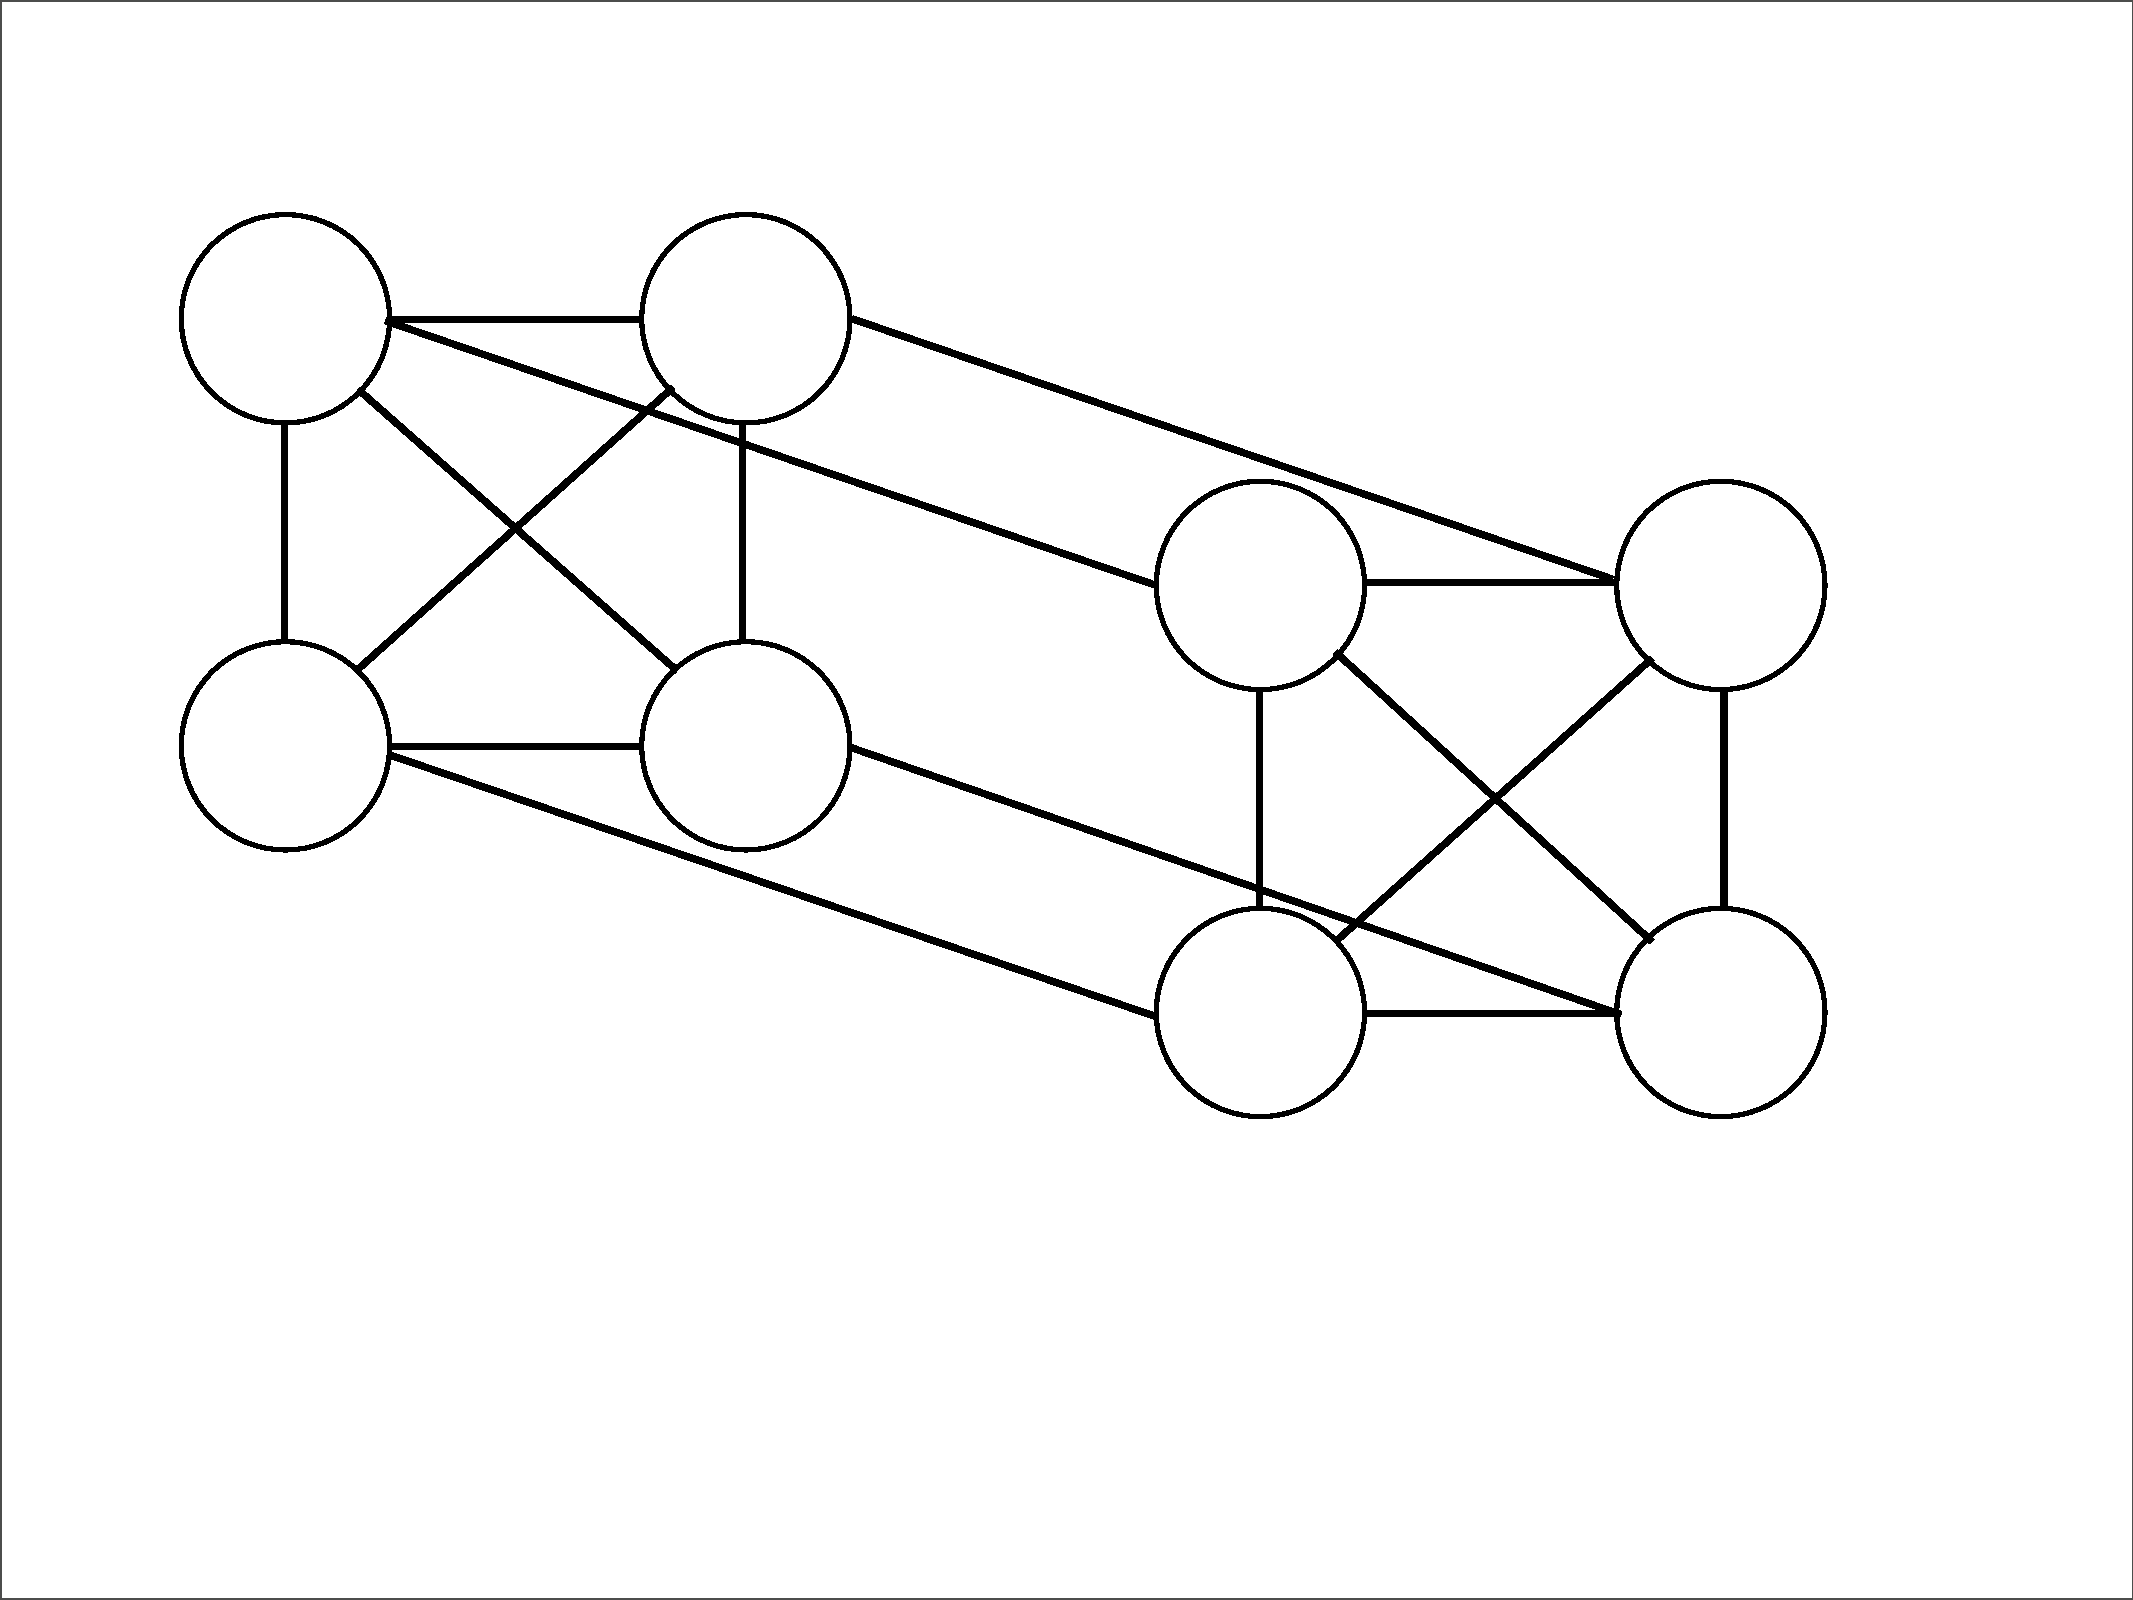
\includegraphics[scale=0.25] {k4xp2.pdf} 
\caption{A $K_4 \times P_2$ Graph }
\label{fig:k4xp2}
\end{figure}


\begin{verbatim}
find nodes : matrix indexed by [int(1..8)] of int(0..16),
       edges: matrix indexed by [int(1..16)] of int(1..16)

such that

|nodes[1] - nodes[2]| = edges[1],
|nodes[1] - nodes[3]| = edges[2],
|nodes[1] - nodes[4]| = edges[3],
|nodes[2] - nodes[3]| = edges[4],
|nodes[2] - nodes[4]| = edges[5],
|nodes[3] - nodes[4]| = edges[6],

|nodes[5] - nodes[6]| = edges[7],
|nodes[5] - nodes[7]| = edges[8],
|nodes[5] - nodes[8]| = edges[9],
|nodes[6] - nodes[7]| = edges[10],
|nodes[6] - nodes[8]| = edges[11],
|nodes[7] - nodes[8]| = edges[12],

|nodes[1] - nodes[5]| = edges[13],
|nodes[2] - nodes[6]| = edges[14],
|nodes[3] - nodes[7]| = edges[15],
|nodes[4] - nodes[8]| = edges[16],

alldiff(edges),
alldiff(nodes)
\end{verbatim}

The Minion model is then:

\begin{verbatim}
MINION 3
\end{verbatim}

There are two 1d arrays of variables one representing all the node variables and one representing all the edge variables. The 8 node variables have domain 0 to 16 and the edge variables have domain 1 to 16. There are also 16 auxiliary variables introduced called aux0 to aux15 there is one of these for each constraint and there is one constraint to represent each edge. 

\begin{verbatim}
**VARIABLES**
DISCRETE nodes[8] {0..16}
DISCRETE edges[16] {1..16}

# auxiliary variables
DISCRETE aux0 {-16..16}
DISCRETE aux1 {-16..16}
DISCRETE aux2 {-16..16}
DISCRETE aux3 {-16..16}
DISCRETE aux4 {-16..16}
DISCRETE aux5 {-16..16}
DISCRETE aux6 {-16..16}
DISCRETE aux7 {-16..16}
DISCRETE aux8 {-16..16}
DISCRETE aux9 {-16..16}
DISCRETE aux10 {-16..16}
DISCRETE aux11 {-16..16}
DISCRETE aux12 {-16..16}
DISCRETE aux13 {-16..16}
DISCRETE aux14 {-16..16}
DISCRETE aux15 {-16..16}
\end{verbatim}

The variable order is to branch on the nodes then on the edges then the auxiliary variables. Only the node and the edge variables are printed. 

\begin{verbatim}
**SEARCH**

PRINT [nodes,edges]

VARORDER [nodes,edges,
aux0,aux1,aux2,aux3,aux4,aux5,aux6,aux7,
aux8,aux9,aux10,aux11,aux12,aux13,aux14,aux15]
\end{verbatim}

Implicit in the problem is an all different constraint on both the node and edge variables. The other constraints are all of the form |nodes[a] - nodes[b]| = edges[a], the first of these constraints from the Essence' specification is $|nodes[1] - nodes[2]| = edges[1]$  this corresponds to the last three constraints in the minion file as the order of constraints are reversed. Minion starts indexing matrices from 0, whereas Essence' started numbering from 1 so the above constraint becomes $|nodes[0] - nodes[1]| = edges[0]$.  This is broken into $nodes[0] - nodes[1] = aux0$ and $|edges[0]| = aux0$. As minion has no weighted sum equals this is broken into a weighted sum less than or equals to and weighted sum greater than or equals to. So this full constraint is represented as $nodes[0] - nodes[1]  \leq aux0$ and $nodes[0] - nodes[1]  \geq aux0$ and $|edges[0]| = aux0$. 

\begin{verbatim}
**CONSTRAINTS**

alldiff([nodes])
alldiff([edges])
weightedsumgeq([1,-1], [nodes[3],nodes[7]], aux15)
weightedsumleq([1,-1], [nodes[3],nodes[7]], aux15)
abs(edges[15],aux15)
weightedsumgeq([1,-1], [nodes[2],nodes[6]], aux14)
weightedsumleq([1,-1], [nodes[2],nodes[6]], aux14)
abs(edges[14],aux14)
weightedsumgeq([1,-1], [nodes[1],nodes[5]], aux13)
weightedsumleq([1,-1], [nodes[1],nodes[5]], aux13)
abs(edges[13],aux13)
weightedsumgeq([1,-1], [nodes[0],nodes[4]], aux12)
weightedsumleq([1,-1], [nodes[0],nodes[4]], aux12)
abs(edges[12],aux12)
weightedsumgeq([1,-1], [nodes[6],nodes[7]], aux11)
weightedsumleq([1,-1], [nodes[6],nodes[7]], aux11)
abs(edges[11],aux11)
weightedsumgeq([1,-1], [nodes[5],nodes[7]], aux10)
weightedsumleq([1,-1], [nodes[5],nodes[7]], aux10)
abs(edges[10],aux10)
weightedsumgeq([1,-1], [nodes[5],nodes[6]], aux9)
weightedsumleq([1,-1], [nodes[5],nodes[6]], aux9)
abs(edges[9],aux9)
weightedsumgeq([1,-1], [nodes[4],nodes[7]], aux8)
weightedsumleq([1,-1], [nodes[4],nodes[7]], aux8)
abs(edges[8],aux8)
weightedsumgeq([1,-1], [nodes[4],nodes[6]], aux7)
weightedsumleq([1,-1], [nodes[4],nodes[6]], aux7)
abs(edges[7],aux7)
weightedsumgeq([1,-1], [nodes[4],nodes[5]], aux6)
weightedsumleq([1,-1], [nodes[4],nodes[5]], aux6)
abs(edges[6],aux6)
weightedsumgeq([1,-1], [nodes[2],nodes[3]], aux5)
weightedsumleq([1,-1], [nodes[2],nodes[3]], aux5)
abs(edges[5],aux5)
weightedsumgeq([1,-1], [nodes[1],nodes[3]], aux4)
weightedsumleq([1,-1], [nodes[1],nodes[3]], aux4)
abs(edges[4],aux4)
weightedsumgeq([1,-1], [nodes[1],nodes[2]], aux3)
weightedsumleq([1,-1], [nodes[1],nodes[2]], aux3)
abs(edges[3],aux3)
weightedsumgeq([1,-1], [nodes[0],nodes[3]], aux2)
weightedsumleq([1,-1], [nodes[0],nodes[3]], aux2)
abs(edges[2],aux2)
weightedsumgeq([1,-1], [nodes[0],nodes[2]], aux1)
weightedsumleq([1,-1], [nodes[0],nodes[2]], aux1)
abs(edges[1],aux1)
weightedsumgeq([1,-1], [nodes[0],nodes[1]], aux0)
weightedsumleq([1,-1], [nodes[0],nodes[1]], aux0)
abs(edges[0],aux0)

**EOF**
\end{verbatim}

\section{The Zebra Puzzle} 

The Zebra Puzzle is a very famous logic puzzle. There are many different versions, but the version we will answer is as follows:
\begin{enumerate}
\item There are five houses.
\item The Englishman lives in the red house.
\item The Spaniard owns the dog.
\item Coffee is drunk in the green house.
\item The Ukrainian drinks tea.
\item The green house is immediately to the right of the ivory house.
\item The Old Gold smoker owns snails.
\item Kools are smoked in the yellow house.
\item Milk is drunk in the middle house.
\item The Norwegian lives in the first house.
\item The man who smokes Chesterfields lives in the house next to the man with the fox.
\item Kools are smoked in the house next to the house where the horse is kept.
\item The Lucky Strike smoker drinks orange juice.
\item The Japanese smokes Parliaments.
\item The Norwegian lives next to the blue house.
\end{enumerate}
Now, who drinks water? Who owns the zebra? In the interest of clarity, it must be added that each of the five houses is painted a different color, and their inhabitants are of different national extractions, own different pets, drink different beverages and smoke different brands of American cigarettes.  These files can be found in /summer\_school/examples the Essence' file is zebra.eprime and the Minion file is zebra.minion. The Essence' specification is as follows:

\begin{verbatim}
language ESSENCE' 1.b.a

$red = colour[1]
$green = colour[2]
$ivory = colour[3]
$yellow = colour[4]
$blue = colour[5]
$Englishman = nationality[1]
$Spaniard = nationality[2]
$Ukranian = nationality[3]
$Norwegian = nationality[4]
$Japanese = nationality[5]
$coffee = drink[1]
$tea = drink[2]
$milk = drink[3]
$orange juice = drink[4]
$Old Gold = smoke[1]
$Kools = smoke[2]
$Chesterfields = smoke[3]
$Lucky Strike = smoke[4]
$Parliaments = smoke[5]
$dog = pets[1]
$snails = pets[2]
$fox = pets[3]
$horse = pets[4]


find colour: matrix indexed by [int(1..5)] of int(1..5),
       nationality: matrix indexed by [int(1..5)] of int(1..5),
       drink: matrix indexed by [int(1..5)] of int(1..5),
       smoke: matrix indexed by [int(1..5)] of int(1..5),
       pets: matrix indexed by [int(1..5)] of int(1..5)

such that

$constraints needed as this is a logical problem where 
$the value allocated to each position of the matrix 
$represents positon of house
alldiff(colour),
alldiff(nationality),
alldiff(drink),
alldiff(smoke),
alldiff(pets),

$There are five houses.
$No constraint covered by domain specification

$The Englishman lives in the red house
nationality[1] = colour[1],

$The Spaniard owns the dog.
nationality[2] = pets[1],

$Coffee is drunk in the green house.
drink[1] = colour[2],

$The Ukranian drinks tea.
nationality[3] = drink[2],

$The green house is immediately to the 
$right of the ivory house.
colour[2] + 1 = colour[3],

$The Old Gold smoker owns snails.
smoke[1] = pets[2],

$Kools are smoked in the yellow house.
smoke[2] = colour[4],

$Milk is drunk in the middle house.
drink[3] = 3,

$The Norwegian lives in the first house
nationality[4] = 1,

$The man who smokes Chesterfields lives in 
$the house next to the man with the fox.
|smoke[3] - pets[3]| = 1,

$Kools are smoked in the house next 
$ to the house where the horse is kept.
|smoke[2] - pets[4]| = 1,

$The Lucky Strike smoker drinks orange juice.
smoke[4] = drink[4],

$The Japanese smokes Parliaments.
nationality[5] = smoke[5],

$The Norwegian lives next to the blue house.
|nationality[4] - colour[5]| = 1

\end{verbatim}

The Minion model is then: 

\begin{verbatim}
MINION 3
\end{verbatim}

There are matrices named colour, nationality, drink, smoke and pets to represent each of the objects discussed in the puzzle. They have domain $\{1,\ldots ,5\}$  which represents where in the row of five houses this object is held. There are also three auxiliary variables introduced which are necessary for the most difficult constraints, these all have domains $\{-4,\ldots ,4\}$.

\begin{verbatim}
**VARIABLES**
DISCRETE colour[5] {1..5}
DISCRETE nationality[5] {1..5}
DISCRETE drink[5] {1..5}
DISCRETE smoke[5] {1..5}
DISCRETE pets[5] {1..5}

# auxiliary variables
DISCRETE aux0 {-4..4}
DISCRETE aux1 {-4..4}
DISCRETE aux2 {-4..4}
\end{verbatim}

The variable order branches on each of the matrices in turn then on the auxiliary variables. Only the matrices of variables are printed.

\begin{verbatim}
**SEARCH**

PRINT [colour,nationality,drink,smoke,pets]

VARORDER [colour,nationality,drink,smoke,pets,aux0,aux1,aux2]
\end{verbatim}

We will go through each constraint in turn. As usual the constraints in Minion are in the reverse order of the Essence' specification and the minion matrices are indexed from 0 whereas 
\begin{verbatim}
**CONSTRAINTS**
\end{verbatim}

$|nationality[4] - colour[5]| = 1$ becomes by counting indices from zero: $|nationality[3] - colour[4]| = 1$. This is then decomposed as $nationality[3] - colour[4] \geq aux2$, $nationality[3] - colour[4] \leq aux2$ and $|aux2|=1$.
\begin{verbatim}
weightedsumgeq([1,-1], [nationality[3],colour[4]], aux2)
weightedsumleq([1,-1], [nationality[3],colour[4]], aux2)
abs(1,aux2)
\end{verbatim}

$nationality[5] = smoke[5]$ becomes by counting indices from zero: $nationality[4] = smoke[4]$.
\begin{verbatim}
eq(nationality[4], smoke[4])
\end{verbatim}

$drink[4] = smoke[4]$ becomes by counting indices from zero: $drink[3] = smoke[3]$.
\begin{verbatim}
eq(drink[3], smoke[3])
\end{verbatim} 

$|smoke[2] - pets[4]| = 1$ becomes by counting indices from zero: $|smoke[1] - pets[3]| = 1$. This is then decomposed as $smoke[1] - pets[3] \leq aux1$, $smoke[1] - pets[3] \geq aux1$ and $|aux1|=1$.
\begin{verbatim}
weightedsumgeq([1,-1], [smoke[1],pets[3]], aux1)
weightedsumleq([1,-1], [smoke[1],pets[3]], aux1)
abs(1,aux1)
\end{verbatim}

$|smoke[3] - pets[3]| = 1$ becomes by counting indices from zero: $|smoke[2] - pets[2]| = 1$. This is then decomposed as $smoke[2] - pets[2] \leq aux0$, $smoke[2] - pets[2] \geq aux0$ and $|aux0|=1$.
\begin{verbatim}
weightedsumgeq([1,-1], [smoke[2],pets[2]], aux0)
weightedsumleq([1,-1], [smoke[2],pets[2]], aux0)
abs(1,aux0)
\end{verbatim}

$nationality[4] = 1$ becomes by counting indices from zero: $nationality[3] = 1$.
\begin{verbatim}
eq(1, nationality[3])
\end{verbatim}

$drink[3] = 3$ becomes by counting indices from zero: $drink[2] = 3$.
\begin{verbatim}
eq(3, drink[2])
\end{verbatim}

$smoke[2] = colour[4]$ becomes by counting indices from zero: $smoke[1] = colour[3]$
\begin{verbatim}
eq(colour[3], smoke[1])
\end{verbatim}

$smoke[1] = pets[2]$ becomes by counting indices from zero: $smoke[0] = pets[1]$
\begin{verbatim}
eq(pets[1], smoke[0])
\end{verbatim}

$colour[2] + 1 = colour[3]$ becomes by counting indices from zero: $colour[1] + 1 = colour[2]$. This is decomposed as $colour[1] + 1 \leq colour[2]$ and $colour[1] + 1 \geq colour[2]$. 
\begin{verbatim}
sumleq([1,colour[1]], colour[2])
sumgeq([1,colour[1]], colour[2])
\end{verbatim}

$nationality[3] = drink[2]$ becomes by counting indices from zero: $nationality[2] = drink[1]$
\begin{verbatim}
eq(drink[1], nationality[2])
\end{verbatim}

$drink[1] = colour[2]$ becomes by counting indices from zero: $drink[0] = colour[1]$
\begin{verbatim}
eq(colour[1], drink[0])
\end{verbatim}

$nationality[2] = pets[1]$ becomes by counting indices from zero: $nationality[1] = pets[0]$
\begin{verbatim}
eq(nationality[1], pets[0])
\end{verbatim}

$nationality[1] = colour[1]$ becomes by counting indices from zero: $nationality[0] = colour[0]$
\begin{verbatim}
eq(colour[0], nationality[0])
\end{verbatim}

There is an implicit all different in the problem which is placed over all the matrices of variables.
\begin{verbatim}
alldiff([pets])
alldiff([smoke])
alldiff([drink])
alldiff([nationality])
alldiff([colour])

**EOF**
\end{verbatim}


\section{N-Queens}
N-Queens is perhaps the most famous problem in CP. It is often used to demonstrate systems. It is stated as  the problem of putting $n$ chess queens on an $n \times n$ chessboard such that none of them is able to capture any other using the standard chess queen's moves. The model we will discuss here is the column model, where there is one variable of domain 1, .. n for each row,  which is the easiest model to describe. We will look at the version where $n=4$ as this has a reasonably small number of constraints to  These files can be found in /summer\_school/examples the Essence' file is NQueensColumn.eprime and the Minion file is NQueensColumn.minion. The Essence' specification is as follows:

\begin{verbatim}
given n: int
find queens: matrix indexed by [int(1..n)] of int(1..n)

such that

forall i : int(1..n). forall j : int(i+1..n).
 |queens[i] - queens[j]| != |i - j|,
 alldiff(queens),

letting n be 4
\end{verbatim}

The Minion model is then: 
\begin{verbatim}
MINION 3
\end{verbatim}

There are 4 variables, each of which represents a column of the chess board. This instance is of a $4 \times 4$ chessboard so there are 4 variables stored in a matrix called queens with domain $\{1,\ldots ,4\}$.  There are two auxiliary variables for each of the 6 diagonal constraints, one with domain $\{-3, \ldots ,3\}$ and one with domain $\{0, \ldots ,3\}$.

\begin{verbatim}
**VARIABLES**
DISCRETE queens[4] {1..4}

# auxiliary variables
DISCRETE aux0 {-3..3}
DISCRETE aux1 {0..3}
DISCRETE aux2 {-3..3}
DISCRETE aux3 {0..3}
DISCRETE aux4 {-3..3}
DISCRETE aux5 {0..3}
DISCRETE aux6 {-3..3}
DISCRETE aux7 {0..3}
DISCRETE aux8 {-3..3}
DISCRETE aux9 {0..3}
DISCRETE aux10 {-3..3}
DISCRETE aux11 {0..3}
\end{verbatim}

The variable order branches on each of the matrice variables in turn then on the auxiliary variables. Only the matrice of variables is printed.
\begin{verbatim}
**SEARCH**

PRINT [queens]

VARORDER [queens,
aux0,aux1,aux2,aux3,aux4,aux5,aux6,aux7,
aux8,aux9,aux10,aux11]
\end{verbatim}

There is an all different constraint on the queens variables. This ensures that two queens cannot be put in the same row. The other constraints stop two queens being placed on a diagonal. These diagonal constraints are all of the form $|queens[i] - queens[j]| \ne |i - j|$.  This is decomposed into the following: $queens[i] - queens[j] = auxa$, $|auxa| = auxb$ and $auxb \ne constant$.  As minion has no weighted sum equals the constraint is broken into a weighted sum less than or equals to and weighted sum greater than or equals to. So this full constraint $queens[i] - queens[j] = auxa$  is represented as $queens[i] - queens[j] \leq auxa$ and $queens[i] - queens[j] \geq auxa$.

\begin{verbatim}
**CONSTRAINTS**

weightedsumgeq([1,-1], [queens[2],queens[3]], aux0)
weightedsumleq([1,-1], [queens[2],queens[3]], aux0)
abs(aux1,aux0)
weightedsumgeq([1,-1], [queens[1],queens[3]], aux2)
weightedsumleq([1,-1], [queens[1],queens[3]], aux2)
abs(aux3,aux2)
weightedsumgeq([1,-1], [queens[1],queens[2]], aux4)
weightedsumleq([1,-1], [queens[1],queens[2]], aux4)
abs(aux5,aux4)
diseq(2, aux3)
weightedsumgeq([1,-1], [queens[0],queens[3]], aux6)
weightedsumleq([1,-1], [queens[0],queens[3]], aux6)
abs(aux7,aux6)
weightedsumgeq([1,-1], [queens[0],queens[2]], aux8)
weightedsumleq([1,-1], [queens[0],queens[2]], aux8)
abs(aux9,aux8)
weightedsumgeq([1,-1], [queens[0],queens[1]], aux10)
weightedsumleq([1,-1], [queens[0],queens[1]], aux10)
abs(aux11,aux10)
diseq(3, aux7)
diseq(2, aux9)
diseq(1, aux1)
diseq(1, aux5)
diseq(1, aux11)
alldiff([queens])

**EOF**
\end{verbatim}

\appendix
\chapter{All the Minion programming constructs}
You are viewing documentation for minion. The same 
documentation is available from a minion executable by 
typing \texttt{minion help} at the command line.
We intend that the command line help system be the 
main source of documentation for the system.

Each of the entries below concerns a different aspect
of the system, and the entries are arranged hierarchically.
For example to view information about the set of available
constraints as a whole view ``constraints'' and to view
specific information about the alldiff constraint view 
``constraints alldiff''.

A good place to start would be viewing the 
``input example'' entry which exhibits a complete
example of a minion input file.

Usage: \texttt{minion [switches] [minion input file]}

\section{constraints}
\paragraph{Description}
{\footnotesize
\begin{verbatim}
  Minion supports many constraints and these are regularly being
  improved and added to. In some cases multiple implementations of the
  same constraints are provided and we would appreciate additional
  feedback on their relative merits in your problem.

  Minion does not support nesting of constraints, however this can be
  achieved by auxiliary variables and reification.

  Variables can be replaced by constants. You can find out more on
  expressions for variables, vectors, etc. in the section on variables.
\end{verbatim}
}
\paragraph{References}
{\footnotesize
\begin{verbatim}
  help variables
\end{verbatim}
}
\section{constraints abs}
\paragraph{Description}
{\footnotesize
\begin{verbatim}
The constraint

   abs(x,y)

makes sure that x=|y|, i.e. x is the absolute value of y.
\end{verbatim}
}
\paragraph{Reference}
{\footnotesize
\begin{verbatim}
help constraints abs
\end{verbatim}
}
\section{constraints alldiff}
\paragraph{Description}
{\footnotesize
\begin{verbatim}
Forces the input vector of variables to take distinct values.
\end{verbatim}
}
\paragraph{Example}
{\footnotesize
\begin{verbatim}
Suppose the input file had the following vector of variables defined:

DISCRETE myVec[9] {1..9}

To ensure that each variable takes a different value include the
following constraint:

alldiff(myVec)
\end{verbatim}
}
\paragraph{Notes}
{\footnotesize
\begin{verbatim}
Enforces the same level of consistency as a clique of not equals 
constraints.
\end{verbatim}
}
\paragraph{References}
{\footnotesize
\begin{verbatim}
See

   help constraints gacalldiff

for the same constraint that enforces GAC.
\end{verbatim}
}
\section{constraints difference}
\paragraph{Description}
{\footnotesize
\begin{verbatim}
The constraint

   difference(x,y,z)

ensures that z=|x-y| in any solution.
\end{verbatim}
}
\paragraph{Notes}
{\footnotesize
\begin{verbatim}
This constraint can be expressed in a much longer form, this form both avoids
requiring an extra variable, and also gets better propagation. It gets bounds
consistency.
\end{verbatim}
}
\section{constraints diseq}
\paragraph{Description}
{\footnotesize
\begin{verbatim}
Constrain two variables to take different values.
\end{verbatim}
}
\paragraph{Notes}
{\footnotesize
\begin{verbatim}
Achieves arc consistency.
\end{verbatim}
}
\paragraph{Example}
{\footnotesize
\begin{verbatim}
diseq(v0,v1)
\end{verbatim}
}
\paragraph{Description}
{\footnotesize
\begin{verbatim}
Constrain two variables to take different values.
\end{verbatim}
}
\paragraph{Notes}
{\footnotesize
\begin{verbatim}
Achieves arc consistency.
\end{verbatim}
}
\paragraph{Example}
{\footnotesize
\begin{verbatim}
diseq(v0,v1)
\end{verbatim}
}
\section{constraints div}
\paragraph{Description}
{\footnotesize
\begin{verbatim}
The constraint
 
   div(x,y,z)

ensures that floor(x/y)=z.

For example:

10/3 = 3
(-10)/3 = -4
10/(-3) = -4
(-10)/(-3) = 3

div and mod satisfy together the condition that:

y*(x/y) + x % y = x

The constraint is always false when y = 0
\end{verbatim}
}
\paragraph{References}
{\footnotesize
\begin{verbatim}
help constraints modulo
\end{verbatim}
}
\section{constraints div\textunderscore undefzero}
\paragraph{Description}
{\footnotesize
\begin{verbatim}
The constraint
 
   div_undefzero(x,y,z)

is the same as div (it ensures that floor(x/y)=z)
except the constraint is always true when y = 0,
instead of false.

This constraint exists for certain special requirements.
In general, if you are unsure what constraint to use,
then what you want is a plain div constraint!
\end{verbatim}
}
\paragraph{References}
{\footnotesize
\begin{verbatim}
help constraints div
\end{verbatim}
}
\section{constraints element}
\paragraph{Description}
{\footnotesize
\begin{verbatim}
The constraint 

   element(vec, i, e)

specifies that, in any solution, vec[i] = e and i is in the range 
[0 .. |vec|-1].
\end{verbatim}
}
\paragraph{Notes}
{\footnotesize
\begin{verbatim}

Warning: This constraint is not confluent. Depending on the order the
propagators are called in Minion, the number of search nodes may vary when
using element. To avoid this problem, use watchelement instead. More details
below.

The level of propagation enforced by this constraint is not named, however it
works as follows. For constraint vec[i]=e:

- After i is assigned, ensures that min(vec[i]) = min(e) and 
  max(vec[i]) = max(e).

- When e is assigned, removes idx from the domain of i whenever e is not an
  element of the domain of vec[idx].

- When m[idx] is assigned, removes idx from i when m[idx] is not in the domain
  of e.

This level of consistency is designed to avoid the propagator having to scan
through vec, except when e is assigned. It does a quantity of cheap propagation
and may work well in practise on certain problems.

Element is not confluent, which may cause the number of search nodes to vary
depending on the order in which constraints are listed in the input file, or 
the order they are called in Minion. For example, the following input causes
Minion to search 41 nodes.

MINION 3
**VARIABLES**
DISCRETE x[5] {1..5}
**CONSTRAINTS**
element([x[0],x[1],x[2]], x[3], x[4])
alldiff([x])
**EOF**

However if the two constraints are swapped over, Minion explores 29 nodes.
As a rule of thumb, to get a lower node count, move element constraints
to the end of the list.
\end{verbatim}
}
\paragraph{References}
{\footnotesize
\begin{verbatim}
See the entry 

   constraints watchelement

for details of an identical constraint that enforces generalised arc
consistency.
\end{verbatim}
}
\section{constraints element\textunderscore one}
\paragraph{Description}
{\footnotesize
\begin{verbatim}
The constraint element one is identical to element, except that the
vector is indexed from 1 rather than from 0.
\end{verbatim}
}
\paragraph{References}
{\footnotesize
\begin{verbatim}
See

   help constraints element

for details of the element constraint which is almost identical to this
one.
\end{verbatim}
}
\section{constraints eq}
\paragraph{Description}
{\footnotesize
\begin{verbatim}
Constrain two variables to take equal values.
\end{verbatim}
}
\paragraph{Example}
{\footnotesize
\begin{verbatim}
eq(x0,x1)
\end{verbatim}
}
\paragraph{Notes}
{\footnotesize
\begin{verbatim}
Achieves bounds consistency.
\end{verbatim}
}
\paragraph{Reference}
{\footnotesize
\begin{verbatim}
help constraints minuseq
\end{verbatim}
}
\paragraph{Description}
{\footnotesize
\begin{verbatim}
Constrain two variables to take equal values.
\end{verbatim}
}
\paragraph{Example}
{\footnotesize
\begin{verbatim}
eq(x0,x1)
\end{verbatim}
}
\paragraph{Notes}
{\footnotesize
\begin{verbatim}
Achieves bounds consistency.
\end{verbatim}
}
\paragraph{Reference}
{\footnotesize
\begin{verbatim}
help constraints minuseq
\end{verbatim}
}
\section{constraints gacalldiff}
\paragraph{Description}
{\footnotesize
\begin{verbatim}
Forces the input vector of variables to take distinct values.
\end{verbatim}
}
\paragraph{Example}
{\footnotesize
\begin{verbatim}
Suppose the input file had the following vector of variables defined:

DISCRETE myVec[9] {1..9}

To ensure that each variable takes a different value include the
following constraint:

gacalldiff(myVec)
\end{verbatim}
}
\paragraph{Notes}
{\footnotesize
\begin{verbatim}
This constraint enforces generalized arc consistency.
\end{verbatim}
}
\section{constraints gacschema}
\paragraph{Description}
{\footnotesize
\begin{verbatim}
An extensional constraint that enforces GAC. The constraint is
specified via a list of tuples.

The format, and usage of gacschema, is identical to the 'table' constraint.
It is difficult to predict which out of 'table' and 'gacschema' will be faster
for any particular problem.
\end{verbatim}
}
\section{constraints gcc}
\paragraph{Description}
{\footnotesize
\begin{verbatim}
The Generalized Cardinality Constraint (GCC) constrains the number of each value
that a set of variables can take.

gcc([primary variables], [values of interest], [capacity variables])

For each value of interest, there must be a capacity variable, which specifies
the number of occurrences of the value in the primary variables.

This constraint only restricts the number of occurrences of the values in
the value list. There is no restriction on the occurrences of other values.
Therefore the semantics of gcc are identical to a set of occurrence 
constraints:

occurrence([primary variables], val1, cap1)
occurrence([primary variables], val2, cap2)
...
\end{verbatim}
}
\paragraph{Example}
{\footnotesize
\begin{verbatim}
Suppose the input file had the following vectors of variables defined:

DISCRETE myVec[9] {1..9}
BOUND cap[9] {0..2}

The following constraint would restrict the occurrence of values 1..9 in myVec
to be at most 2 each initially, and finally equal to the values of the cap
vector.

gcc(myVec, [1,2,3,4,5,6,7,8,9], cap)
\end{verbatim}
}
\paragraph{Notes}
{\footnotesize
\begin{verbatim}
This constraint enforces a hybrid consistency. It reads the bounds of the
capacity variables, then enforces GAC over the primary variables only.  Then the
bounds of the capacity variables are updated using flow algorithms similar to
those proposed by Quimper et al, Improved Algorithms for the Global Cardinality
Constraint (CP 2004).

This constraint provides stronger propagation to the capacity variables than the
gccweak constraint.
\end{verbatim}
}
\section{constraints gccweak}
\paragraph{Description}
{\footnotesize
\begin{verbatim}
The Generalized Cardinality Constraint (GCC) (weak variant) constrains the 
number of each value that a set of variables can take.

gccweak([primary variables], [values of interest], [capacity variables])

For each value of interest, there must be a capacity variable, which specifies
the number of occurrences of the value in the primary variables.

This constraint only restricts the number of occurrences of the values in
the value list. There is no restriction on the occurrences of other values.
Therefore the semantics of gccweak are identical to a set of occurrence 
constraints:

occurrence([primary variables], val1, cap1)
occurrence([primary variables], val2, cap2)
...
\end{verbatim}
}
\paragraph{Example}
{\footnotesize
\begin{verbatim}
Suppose the input file had the following vectors of variables defined:

DISCRETE myVec[9] {1..9}
BOUND cap[9] {0..2}

The following constraint would restrict the occurrence of values 1..9 in myVec
to be at most 2 each initially, and finally equal to the values of the cap
vector.

gccweak(myVec, [1,2,3,4,5,6,7,8,9], cap)
\end{verbatim}
}
\paragraph{Notes}
{\footnotesize
\begin{verbatim}
This constraint enforces a hybrid consistency. It reads the bounds of the
capacity variables, then enforces GAC over the primary variables only.  Then the
bounds of the capacity variables are updated by counting values in the domains
of the primary variables.

The consistency over the capacity variables is weaker than the gcc constraint, 
hence the name gccweak.
\end{verbatim}
}
\section{constraints haggisgac}
\paragraph{Description}
{\footnotesize
\begin{verbatim}
An extensional constraint that enforces GAC. This constraint make uses
of 'short tuples', which allow some values to be marked as don't care.
When this allows the set of tuples to be reduced in size, this leads to
performance gains.

The variables used in the constraint have to be BOOL or DISCRETE variables.
Other types are not supported.
\end{verbatim}
}
\paragraph{Example}
{\footnotesize
\begin{verbatim}

Consider the constraint 'min([x1,x2,x3],x4)'' on Booleans variables
x1,x2,x3,x4.

Represented as a TUPLELIST for a table or gacschema constraint, this would
look like:

**TUPLELIST**
mycon 8 4
0 0 0 0
0 0 1 0
0 1 0 0
0 1 1 0
1 0 0 0
1 0 1 0
1 1 0 0
1 1 1 1

Short tuples give us a way of shrinking this list. Short tuples consist
of pairs (x,y), where x is a varible position, and y is a value for that 
variable. For example:

[(0,0),(3,0)]

Represents 'If the variable at index 0 is 0, and the variable at index
3 is 0, then the constraint is true'.

This allows us to represent our constraint as follows:

**SHORTTUPLELIST**
mycon 4
[(0,0),(3,0)]
[(1,0),(3,0)]
[(2,0),(3,0)]
[(0,1),(1,1),(2,1),(3,1)]

Note that some tuples are double-represented here. The first 3 short
tuples all allow the assignment '0 0 0 0'. This is fine. The important
thing for efficency is to try to give a small list of short tuples.


We use this tuple by writing:

haggisgac([x1,x2,x3,x4], mycon)

and now the variables [x1,x2,x3,x4] will satisfy the constraint mycon.
\end{verbatim}
}
\paragraph{References}
{\footnotesize
\begin{verbatim}
help input shorttuplelist
help constraints table
help constraints negativetable
help constraints shortstr2
\end{verbatim}
}
\section{constraints haggisgac-stable}
\paragraph{Description}
{\footnotesize
\begin{verbatim}
An extensional constraint that enforces GAC. haggisgac-stable
is a variant of haggisgac which uses less memory in some cases,
and can also be faster (or slower). The input is identical to
haggisgac.
\end{verbatim}
}
\paragraph{References}
{\footnotesize
\begin{verbatim}
help constraints haggisgac
\end{verbatim}
}
\section{constraints hamming}
\paragraph{Description}
{\footnotesize
\begin{verbatim}
The constraint

   hamming(X,Y,c)

ensures that the hamming distance between X and Y is at least c. That is, that
the size of the set {i | X[i] != y[i]} is greater than or equal to c.
\end{verbatim}
}
\section{constraints ineq}
\paragraph{Description}
{\footnotesize
\begin{verbatim}
The constraint

   ineq(x, y, k)

ensures that 

   x <= y + k 

in any solution.
\end{verbatim}
}
\paragraph{Notes}
{\footnotesize
\begin{verbatim}
Minion has no strict inequality (<) constraints. However x < y can be
achieved by

   ineq(x, y, -1)
\end{verbatim}
}
\section{constraints lexleq}
\paragraph{Description}
{\footnotesize
\begin{verbatim}
The constraint

   lexleq(vec0, vec1)

takes two vectors vec0 and vec1 of the same length and ensures that
vec0 is lexicographically less than or equal to vec1 in any solution.
\end{verbatim}
}
\paragraph{Notes}
{\footnotesize
\begin{verbatim}
This constraints achieves GAC.
\end{verbatim}
}
\paragraph{References}
{\footnotesize
\begin{verbatim}
See also

   help constraints lexless

for a similar constraint with strict lexicographic inequality.
\end{verbatim}
}
\section{constraints lexleq[rv]}
\paragraph{Description}
{\footnotesize
\begin{verbatim}
  The constraint

  lexle[rv](vec0, vec1)

  takes two vectors vec0 and vec1 of the same length and ensures that
  vec0 is lexicographically less than or equal to vec1 in any solution.
\end{verbatim}
}
\paragraph{Notes}
{\footnotesize
\begin{verbatim}
  This constraint achieves GAC even when some variables are repeated in
  vec0 and vec1. However, the extra propagation this achieves is rarely 
  worth the extra work.
\end{verbatim}
}
\paragraph{References}
{\footnotesize
\begin{verbatim}
  See also

  help constraints lexleq[quick]

  for a much faster logically identical constraint, with lower
  propagation.
\end{verbatim}
}
\section{constraints lexless}
\paragraph{Description}
{\footnotesize
\begin{verbatim}
The constraint

   lexless(vec0, vec1)

takes two vectors vec0 and vec1 of the same length and ensures that
vec0 is lexicographically less than vec1 in any solution.
\end{verbatim}
}
\paragraph{Notes}
{\footnotesize
\begin{verbatim}
This constraint maintains GAC.
\end{verbatim}
}
\paragraph{References}
{\footnotesize
\begin{verbatim}
See also

   help constraints lexleq

for a similar constraint with non-strict lexicographic inequality.
\end{verbatim}
}
\section{constraints lighttable}
\paragraph{Description}
{\footnotesize
\begin{verbatim}
An extensional constraint that enforces GAC. The constraint is
specified via a list of tuples. lighttable is a variant of the 
table constraint that is stateless and potentially faster
for small constraints.

For full documentation, see the help for the table constraint.
\end{verbatim}
}
\section{constraints litsumgeq}
\paragraph{Description}
{\footnotesize
\begin{verbatim}
The constraint litsumgeq(vec1, vec2, c) ensures that there exists at least c
distinct indices i such that vec1[i] = vec2[i].
\end{verbatim}
}
\paragraph{Notes}
{\footnotesize
\begin{verbatim}
A SAT clause {x,y,z} can be created using:

   litsumgeq([x,y,z],[1,1,1],1)

Note also that this constraint is more efficient for smaller values of c. For
large values consider using watchsumleq.
\end{verbatim}
}
\paragraph{Reifiability}
{\footnotesize
\begin{verbatim}
This constraint is not reifiable.
\end{verbatim}
}
\paragraph{References}
{\footnotesize
\begin{verbatim}
See also

   help constraints watchsumleq
   help constraints watchsumgeq
\end{verbatim}
}
\section{constraints max}
\paragraph{Description}
{\footnotesize
\begin{verbatim}
The constraint

   max(vec, x)

ensures that x is equal to the maximum value of any variable in vec.
\end{verbatim}
}
\paragraph{References}
{\footnotesize
\begin{verbatim}
See

   help constraints min

for the opposite constraint.
\end{verbatim}
}
\section{constraints mddc}
\paragraph{Description}
{\footnotesize
\begin{verbatim}
MDDC (mddc) is an implementation of MDDC(sp) by Cheng and Yap. It enforces GAC on a 
constraint using a multi-valued decision diagram (MDD). 

The MDD required for the propagator is constructed from a set of satisfying
tuples. The constraint has the same syntax as 'table' and can function
as a drop-in replacement. 

For examples on how to call it, see the help for 'table'. Substitute 'mddc' for
'table'.
\end{verbatim}
}
\paragraph{Notes}
{\footnotesize
\begin{verbatim}
This constraint enforces generalized arc consistency.
\end{verbatim}
}
\section{constraints min}
\paragraph{Description}
{\footnotesize
\begin{verbatim}
The constraint

   min(vec, x)

ensures that x is equal to the minimum value of any variable in vec.
\end{verbatim}
}
\paragraph{References}
{\footnotesize
\begin{verbatim}
See

   help constraints max

for the opposite constraint.
\end{verbatim}
}
\section{constraints minuseq}
\paragraph{Description}
{\footnotesize
\begin{verbatim}
Constraint

   minuseq(x,y)

ensures that x=-y.
\end{verbatim}
}
\paragraph{Reference}
{\footnotesize
\begin{verbatim}
help constraints eq
\end{verbatim}
}
\paragraph{Description}
{\footnotesize
\begin{verbatim}
Constraint

   minuseq(x,y)

ensures that x=-y.
\end{verbatim}
}
\paragraph{Reference}
{\footnotesize
\begin{verbatim}
help constraints eq
\end{verbatim}
}
\section{constraints modulo}
\paragraph{Description}
{\footnotesize
\begin{verbatim}
The constraint
 
   modulo(x,y,z)

ensures that x%y=z i.e. z is the remainder of dividing x by y.
For negative values, we ensure that:

y(x/y) + x%y = x

To be fully concrete, here are some examples:

3 % 5 = 3
-3 % 5 = 2
3 % -5 = -2
-3 % -5 = -3
\end{verbatim}
}
\paragraph{References}
{\footnotesize
\begin{verbatim}
help constraints div
\end{verbatim}
}
\section{constraints mod\textunderscore undefzero}
\paragraph{Description}
{\footnotesize
\begin{verbatim}
The constraint
 
   mod_undefzero(x,y,z)

is the same as mod except the constraint is always 
true when y = 0, instead of false.

This constraint exists for certain special requirements.
In general, if you are unsure what constraint to use,
then what you want is a plain mod constraint!
\end{verbatim}
}
\paragraph{References}
{\footnotesize
\begin{verbatim}
help constraints mod
\end{verbatim}
}
\section{constraints negativemddc}
\paragraph{Description}
{\footnotesize
\begin{verbatim}
Negative MDDC (negativemddc) is an implementation of MDDC(sp) by Cheng and Yap. 
It enforces GAC on a constraint using a multi-valued decision diagram (MDD). 

The MDD required for the propagator is constructed from a set of unsatisfying
(negative) tuples. The constraint has the same syntax as 'negativetable' and
can function as a drop-in replacement. 
\end{verbatim}
}
\paragraph{Notes}
{\footnotesize
\begin{verbatim}
This constraint enforces generalized arc consistency.
\end{verbatim}
}
\section{constraints negativetable}
\paragraph{Description}
{\footnotesize
\begin{verbatim}
An extensional constraint that enforces GAC. The constraint is
specified via a list of disallowed tuples.
\end{verbatim}
}
\paragraph{Notes}
{\footnotesize
\begin{verbatim}
See entry 

   help input negativetable

for how to specify a table constraint in minion input. The only
difference for negativetable is that the specified tuples are
disallowed.
\end{verbatim}
}
\paragraph{References}
{\footnotesize
\begin{verbatim}
help input table
help input tuplelist
\end{verbatim}
}
\section{constraints occurrence}
\paragraph{Description}
{\footnotesize
\begin{verbatim}
The constraint

   occurrence(vec, elem, count)

ensures that there are count occurrences of the value elem in the
vector vec.
\end{verbatim}
}
\paragraph{Notes}
{\footnotesize
\begin{verbatim}
elem must be a constant, not a variable.
\end{verbatim}
}
\paragraph{References}
{\footnotesize
\begin{verbatim}
help constraints occurrenceleq
help constraints occurrencegeq
\end{verbatim}
}
\section{constraints occurrencegeq}
\paragraph{Description}
{\footnotesize
\begin{verbatim}
The constraint

   occurrencegeq(vec, elem, count)

ensures that there are AT LEAST count occurrences of the value elem in
the vector vec.
\end{verbatim}
}
\paragraph{Notes}
{\footnotesize
\begin{verbatim}
elem and count must be constants
\end{verbatim}
}
\paragraph{References}
{\footnotesize
\begin{verbatim}
help constraints occurrence
help constraints occurrenceleq
\end{verbatim}
}
\section{constraints occurrenceleq}
\paragraph{Description}
{\footnotesize
\begin{verbatim}
The constraint

   occurrenceleq(vec, elem, count)

ensures that there are AT MOST count occurrences of the value elem in
the vector vec.
\end{verbatim}
}
\paragraph{Notes}
{\footnotesize
\begin{verbatim}
elem and count must be constants
\end{verbatim}
}
\paragraph{References}
{\footnotesize
\begin{verbatim}
help constraints occurrence
help constraints occurrencegeq
\end{verbatim}
}
\section{constraints pow}
\paragraph{Description}
{\footnotesize
\begin{verbatim}
The constraint
 
   pow(x,y,z)

ensures that x^y=z.
\end{verbatim}
}
\paragraph{Notes}
{\footnotesize
\begin{verbatim}
This constraint is only available for positive domains x, y and z.
\end{verbatim}
}
\section{constraints product}
\paragraph{Description}
{\footnotesize
\begin{verbatim}
The constraint

   product(x,y,z)

ensures that z=xy in any solution.
\end{verbatim}
}
\paragraph{Notes}
{\footnotesize
\begin{verbatim}
This constraint can be used for (and, in fact, has a specialised
implementation for) achieving boolean AND, i.e. x & y=z can be modelled
as

   product(x,y,z)

The general constraint achieves bounds generalised arc consistency for
positive numbers.
\end{verbatim}
}
\section{constraints reification}
\paragraph{Description}
{\footnotesize
\begin{verbatim}
Reification is provided in two forms: reify and reifyimply.

   reify(constraint, r) where r is a 0/1 var

ensures that r is set to 1 if and only if constraint is satisfied. That is, if r
is 0 the constraint must NOT be satisfied; and if r is 1 it must be satisfied as
normal. Conversely, if the constraint is satisfied then r must be 1, and if not
then r must be 0.

   reifyimply(constraint, r)

only checks that if r is set to 1 then constraint must be satisfied. If r is not
1, constraint may be either satisfied or unsatisfied. Furthermore r is never set
by propagation, only by search; that is, satisfaction of constraint does not
affect the value of r.
\end{verbatim}
}
\paragraph{Notes}
{\footnotesize
\begin{verbatim}
ALMOST ALL constraints are are reifiable. Individual constraint entries mention
if the constraint is NOT reifiable.

ALL constraints are reifyimplyable.
\end{verbatim}
}
\section{constraints reify}
\paragraph{References}
{\footnotesize
\begin{verbatim}
See
   help constraints reification
\end{verbatim}
}
\section{constraints reifyimply}
\paragraph{References}
{\footnotesize
\begin{verbatim}
See
   help constraints reification
\end{verbatim}
}
\section{constraints shortstr2}
\paragraph{Description}
{\footnotesize
\begin{verbatim}
ShortSTR2 is the algorithm described in the IJCAI 2013 paper by Jefferson and
Nightingale. It is an extension of STR2+ by Christophe Lecoutre, adapted for
short supports. 
\end{verbatim}
}
\paragraph{Example}
{\footnotesize
\begin{verbatim}

Input format is exactly the same as haggisgac. Refer to the haggisgac and
shorttuplelist pages for more information. 

Example:

**SHORTTUPLELIST**
mycon 4
[(0,0),(3,0)]
[(1,0),(3,0)]
[(2,0),(3,0)]
[(0,1),(1,1),(2,1),(3,1)]

**CONSTRAINTS**
shortstr2([x1,x2,x3,x4], mycon)
\end{verbatim}
}
\paragraph{Notes}
{\footnotesize
\begin{verbatim}
This constraint enforces generalized arc consistency.
\end{verbatim}
}
\paragraph{References}
{\footnotesize
\begin{verbatim}
help input shorttuplelist
help constraints table
help constraints negativetable
help constraints haggisgac
help constraints haggisgac-stable
\end{verbatim}
}
\paragraph{Notes}
{\footnotesize
\begin{verbatim}
This constraint enforces generalized arc consistency.
\end{verbatim}
}
\section{constraints str2plus}
\paragraph{Description}
{\footnotesize
\begin{verbatim}
str2plus is an implementation of the STR2+ algorithm by Christophe Lecoutre.
\end{verbatim}
}
\paragraph{Example}
{\footnotesize
\begin{verbatim}

str2plus is invoked in the same way as all other table constraints, such 
as table and mddc.

str2plus([x,y,z], {<1,2,3>, <1,3,2>})
\end{verbatim}
}
\section{constraints sumgeq}
\paragraph{Description}
{\footnotesize
\begin{verbatim}
The constraint

   sumgeq(vec, c)

ensures that sum(vec) >= c.
\end{verbatim}
}
\section{constraints sumleq}
\paragraph{Description}
{\footnotesize
\begin{verbatim}
The constraint

   sumleq(vec, c)

ensures that sum(vec) <= c.
\end{verbatim}
}
\section{constraints table}
\paragraph{Description}
{\footnotesize
\begin{verbatim}
An extensional constraint that enforces GAC. The constraint is
specified via a list of tuples.

The variables used in the constraint have to be BOOL or DISCRETE variables.
Other types are not supported.
\end{verbatim}
}
\paragraph{Example}
{\footnotesize
\begin{verbatim}
To specify a constraint over 3 variables that allows assignments
(0,0,0), (1,0,0), (0,1,0) or (0,0,1) do the following.

1) Add a tuplelist to the **TUPLELIST** section, e.g.:

**TUPLELIST**
myext 4 3
0 0 0
1 0 0
0 1 0
0 0 1

N.B. the number 4 is the number of tuples in the constraint, the 
number 3 is the -arity.

2) Add a table constraint to the **CONSTRAINTS** section, e.g.:

**CONSTRAINTS**
table(myvec, myext)

and now the variables of myvec will satisfy the constraint myext.
\end{verbatim}
}
\paragraph{Example}
{\footnotesize
\begin{verbatim}
The constraints extension can also be specified in the constraint
definition, e.g.:

table(myvec, {<0,0,0>,<1,0,0>,<0,1,0>,<0,0,1>})
\end{verbatim}
}
\paragraph{References}
{\footnotesize
\begin{verbatim}
help input tuplelist
help input gacschema
help input negativetable
help input haggisgac
\end{verbatim}
}
\paragraph{References}
{\footnotesize
\begin{verbatim}
help input tuplelist
help input table
help input haggisgac
\end{verbatim}
}
\section{constraints watched-and}
\paragraph{Description}
{\footnotesize
\begin{verbatim}
The constraint

  watched-and({C1,...,Cn})

ensures that the constraints C1,...,Cn are all true.
\end{verbatim}
}
\paragraph{Notes}
{\footnotesize
\begin{verbatim}
pointless, bearing in mind that a CSP is simply a conjunction of constraints
already! However sometimes it may be necessary to use a conjunction as a child
of another constraint, for example in a reification:

   reify(watched-and({...}),r)
\end{verbatim}
}
\paragraph{References}
{\footnotesize
\begin{verbatim}
  See also

  help constraints watched-or
\end{verbatim}
}
\section{constraints watched-or}
\paragraph{Description}
{\footnotesize
\begin{verbatim}
The constraint

  watched-or({C1,...,Cn})

ensures that at least one of the constraints C1,...,Cn is true.
\end{verbatim}
}
\paragraph{References}
{\footnotesize
\begin{verbatim}
  See also

  help constraints watched-and
\end{verbatim}
}
\section{constraints watchelement}
\paragraph{Description}
{\footnotesize
\begin{verbatim}
The constraint 

   watchelement(vec, i, e)

specifies that, in any solution, vec[i] = e and i is in the range 
[0 .. |vec|-1].
\end{verbatim}
}
\paragraph{Notes}
{\footnotesize
\begin{verbatim}
Enforces generalised arc consistency.
\end{verbatim}
}
\paragraph{References}
{\footnotesize
\begin{verbatim}
See entry

   help constraints element

for details of an identical constraint that enforces a lower level of
consistency.
\end{verbatim}
}
\section{constraints watchelement\textunderscore one}
\paragraph{Description}
{\footnotesize
\begin{verbatim}
This constraint is identical to watchelement, except the vector
is indexed from 1 rather than from 0.
\end{verbatim}
}
\paragraph{References}
{\footnotesize
\begin{verbatim}
See entry

   help constraints watchelement

for details of watchelement which watchelement_one is based on.
\end{verbatim}
}
\section{constraints watchelement\textunderscore undefzero}
\paragraph{Description}
{\footnotesize
\begin{verbatim}
The constraint 

   watchelement_undefzero(vec, i, e)

specifies that, in any solution, either:
a)  vec[i] = e and i is in the range [0 .. |vec|-1]
b)  i is outside the index range of vec, and e = 0

Unlike watchelement (and element) which are false if i is outside
the index range of vec.

In general, use watchelement unless you have a special reason to
use this constraint!
\end{verbatim}
}
\paragraph{Notes}
{\footnotesize
\begin{verbatim}
Enforces generalised arc consistency.
\end{verbatim}
}
\paragraph{References}
{\footnotesize
\begin{verbatim}
See entry

   help constraints watchelement

for details of the standard element constraint, which is false
when the array value is out of bounds.
\end{verbatim}
}
\section{constraints watchless}
\paragraph{Description}
{\footnotesize
\begin{verbatim}
The constraint watchless(x,y) ensures that x is less than y.
\end{verbatim}
}
\paragraph{References}
{\footnotesize
\begin{verbatim}
  See also

  help constraints ineq
\end{verbatim}
}
\section{constraints watchsumgeq}
\paragraph{Description}
{\footnotesize
\begin{verbatim}
  The constraint watchsumgeq(vec, c) ensures that sum(vec) >= c.
\end{verbatim}
}
\paragraph{Notes}
{\footnotesize
\begin{verbatim}
  For this constraint, small values of c are more efficient.

  Equivalent to litsumgeq(vec, [1,...,1], c), but faster.

  This constraint works on 0/1 variables only.
\end{verbatim}
}
\paragraph{Reifiability}
{\footnotesize
\begin{verbatim}
  This constraint is not reifiable.
\end{verbatim}
}
\paragraph{References}
{\footnotesize
\begin{verbatim}
  See also

  help constraints watchsumleq 
  help constraints litsumgeq
\end{verbatim}
}
\section{constraints watchsumleq}
\paragraph{Description}
{\footnotesize
\begin{verbatim}
  The constraint watchsumleq(vec, c) ensures that sum(vec) <= c.
\end{verbatim}
}
\paragraph{Notes}
{\footnotesize
\begin{verbatim}
  Equivalent to litsumgeq([vec1,...,vecn], [0,...,0], n-c) but faster.

  This constraint works on binary variables only.

  For this constraint, large values of c are more efficient.
\end{verbatim}
}
\paragraph{References}
{\footnotesize
\begin{verbatim}
  See also

  help constraints watchsumgeq 
  help constraints litsumgeq
\end{verbatim}
}
\section{constraints watchvecneq}
\paragraph{Description}
{\footnotesize
\begin{verbatim}
The constraint

   watchvecneq(A, B)

ensures that A and B are not the same vector, i.e., there exists some index i
such that A[i] != B[i].
\end{verbatim}
}
\section{constraints weightedsumgeq}
\paragraph{Description}
{\footnotesize
\begin{verbatim}
The constraint

   weightedsumgeq(constantVec, varVec, total)

ensures that constantVec.varVec >= total, where constantVec.varVec is
the scalar dot product of constantVec and varVec.
\end{verbatim}
}
\paragraph{References}
{\footnotesize
\begin{verbatim}
help constraints weightedsumleq
help constraints sumleq
help constraints sumgeq
\end{verbatim}
}
\section{constraints weightedsumleq}
\paragraph{Description}
{\footnotesize
\begin{verbatim}
The constraint

   weightedsumleq(constantVec, varVec, total)

ensures that constantVec.varVec <= total, where constantVec.varVec is
the scalar dot product of constantVec and varVec.
\end{verbatim}
}
\paragraph{References}
{\footnotesize
\begin{verbatim}
help constraints weightedsumgeq
help constraints sumleq
help constraints sumgeq
\end{verbatim}
}
\section{constraints w-inrange}
\paragraph{Description}
{\footnotesize
\begin{verbatim}
  The constraint w-inrange(x, [a,b]) ensures that a <= x <= b.
\end{verbatim}
}
\paragraph{References}
{\footnotesize
\begin{verbatim}
  See also

  help constraints w-notinrange
\end{verbatim}
}
\section{constraints w-inset}
\paragraph{Description}
{\footnotesize
\begin{verbatim}
The constraint w-inset(x, [a1,...,an]) ensures that x belongs to the set 
{a1,..,an}.
\end{verbatim}
}
\paragraph{References}
{\footnotesize
\begin{verbatim}
  See also

  help constraints w-notinset
\end{verbatim}
}
\paragraph{Description}
{\footnotesize
\begin{verbatim}
The constraint w-inintervalset(x, [a1,a2, b1,b2, ... ]) ensures that the value 
of x belongs to one of the intervals  {a1,...,a2}, {b1,...,b2} etc. The list of 
intervals must be given in numerical order. 
\end{verbatim}
}
\paragraph{References}
{\footnotesize
\begin{verbatim}
  See also

  help constraints w-notinset
\end{verbatim}
}
\section{constraints w-literal}
\paragraph{Description}
{\footnotesize
\begin{verbatim}
  The constraint w-literal(x, a) ensures that x=a.
\end{verbatim}
}
\paragraph{References}
{\footnotesize
\begin{verbatim}
  See also

  help constraints w-notliteral
\end{verbatim}
}
\section{constraints w-notinrange}
\paragraph{Description}
{\footnotesize
\begin{verbatim}
  The constraint w-notinrange(x, [a,b]) ensures that x < a or b < x.
\end{verbatim}
}
\paragraph{References}
{\footnotesize
\begin{verbatim}
  See also

  help constraints w-inrange
\end{verbatim}
}
\section{constraints w-notinset}
\paragraph{Description}
{\footnotesize
\begin{verbatim}
The constraint w-notinset(x, [a1,...,an]) ensures that x does not belong to the
set {a1,..,an}.
\end{verbatim}
}
\paragraph{References}
{\footnotesize
\begin{verbatim}
  See also

  help constraints w-inset
\end{verbatim}
}
\section{constraints w-notliteral}
\paragraph{Description}
{\footnotesize
\begin{verbatim}
  The constraint w-notliteral(x, a) ensures that x =/= a.
\end{verbatim}
}
\paragraph{References}
{\footnotesize
\begin{verbatim}
  See also

  help constraints w-literal
\end{verbatim}
}
\section{input}
\paragraph{Description}
{\footnotesize
\begin{verbatim}

Minion expects to be provided with the name of an input file as an
argument. This file contains a specification of the CSP to be solved
as well as settings that the search process should use. The format is

Minion3Input::= MINION 3
                <InputSection>+
                **EOF**

InputSection::= <VariablesSection> 
              | <SearchSection>
              | <ConstraintsSection> 
              | <TuplelistSection>
              | <ShortTuplelistSection>

i.e. 'MINION 3' followed by any number of variable, search,
constraints and tuplelists sections (can repeat) followed by
'**EOF**', the end of file marker.

All text from a '#' character to the end of the line is ignored.

See the associated help entries below for information on each section.
\end{verbatim}
}
\paragraph{Notes}
{\footnotesize
\begin{verbatim}
You can give an input file via standard input by specifying '--' as the file
name, this might help when minion is being used as a tool in a shell script or
for compressed input, e.g.,

   gunzip -c myinput.minion.gz | minion
\end{verbatim}
}
\section{input constraints}
\paragraph{Description}
{\footnotesize
\begin{verbatim}

The constraints section consists of any number of constraint
declarations on separate lines.

ConstraintsSection::= **CONSTRAINTS**
                      <ConstraintDeclaration>*
\end{verbatim}
}
\paragraph{Example}
{\footnotesize
\begin{verbatim}
**CONSTRAINTS**
eq(bool,0)
alldiff(d)
\end{verbatim}
}
\paragraph{References}
{\footnotesize
\begin{verbatim}
See help entries for individual constraints under

   help constraints

for details on constraint declarations.
\end{verbatim}
}
\section{input example}
\paragraph{Example}
{\footnotesize
\begin{verbatim}
Below is a complete minion input file with commentary, as an example.

MINION 3

# While the variable section doesn't have to come first, you can't 
# really do anything until
# You have one...
**VARIABLES**

# There are 4 type of variables
BOOL bool         # Boolean don't need a domain
BOUND b {1..3}    # Bound vars need a domain given as a range
DISCRETE d {1..3} # So do discrete vars

#Note: Names are case sensitive!

# Internally, Bound variables are stored only as a lower and upper bound
# Whereas discrete variables allow any sub-domain

SPARSEBOUND s {1,3,6,7} # Sparse bound variables take a sorted list of values

# We can also declare matrices of variables!

DISCRETE q[3] {0..5} # This is a matrix with 3 variables: q[0],q[1] and q[2]
BOOL bm[2,2] # A 2d matrix, variables bm[0,0], bm[0,1], bm[1,0], bm[1,1]
BOOL bn[2,2,2,2] # You can have as many indices as you like!

#The search section is entirely optional
**SEARCH**

# Note that everything in SEARCH is optional, and can only be given at
# most once!

# If you don't give an explicit variable ordering, one is generated.
# These can take matrices in interesting ways like constraints, see below.
VARORDER [bool,b,d]

# If you don't give a value ordering, 'ascending' is used
#VALORDER [a,a,a,a]

# You can have one objective function, or none at all.
MAXIMISING bool
# MINIMISING x3

# both (MAX/MIN)IMISING and (MAX/MIN)IMIZING are accepted...


# Print statement takes a vector of things to print

PRINT [bool, q]

# You can also give:
# PRINT ALL (the default)
# PRINT NONE


# Declare constraints in this section!
**CONSTRAINTS**

# Constraints are defined in exactly the same way as in MINION input
formats 1 & 2
eq(bool, 0)
eq(b,d)

# To get a single variable from a matrix, just index it
eq(q[1],0)
eq(bn[0,1,1,1], bm[1,1])

# It's easy to get a row or column from a matrix. Just use _ in the
# indices you want
# to vary. Just giving a matrix gives all the variables in that matrix.

#The following shows how flattening occurs...

# [bm] == [ bm[_,_] ] == [ bm[0,0], bm[0,1], bm[1,0], bm[1,1] ]
# [ bm[_,1] ] = [ bm[0,1], bm[1,1] ]
# [ bn[1,_,0,_] = [ bn[1,0,0,0], b[1,0,0,1], b[1,1,0,0], b[1,1,0,1] ]

# You can string together a list of such expressions!

lexleq( [bn[1,_,0,_], bool, q[0]] , [b, bm, d] )

# One minor problem.. you must always put [ ] around any matrix expression, so
# lexleq(bm, bm) is invalid

lexleq( [bm], [bm] ) # This is OK!

# Can give tuplelists, which can have names!
# The input is: <name> <num_of_tuples> <tuple_length> <numbers...>
# The formatting can be about anything..

**TUPLELIST**

Fred 3 3
0 2 3
2 0 3
3 1 3

Bob 2 2 1 2 3 4

#No need to put everything in one section! All sections can be reopened..
**VARIABLES**

# You can even have empty sections.. if you want

**CONSTRAINTS**

#Specify tables by their names..

table([q], Fred)

# Can still list tuples explicitally in the constraint if you want at
# the moment.
# On the other hand, I might remove this altogether, as it's worse than giving
# Tuplelists

table([q],{ <0,2,3>,<2,0,3>,<3,1,3> })

#Must end with the **EOF** marker!

**EOF**

Any text down here is ignored, so you can write whatever you like (or
nothing at all...)
\end{verbatim}
}
\section{input search}
\paragraph{Description}
{\footnotesize
\begin{verbatim}

Inside the search section one can specify

- variable orderings, 
- value orderings,
- optimisation function, and
- details of how to print out solutions.

   SearchSection::= <VarValOrdering>*
                    <OptimisationFn>?
                    <PrintFormat>?

If no varval ordering is given then the variables are assigned in instantiation
order and the values tried in ascending order.

If a variable order is given as a command line argument it will override
anything specified in the input file.

Multiple variable orders can be given, each with an optional value ordering:

   VarValOrdering::= <VarOrder> 
                     <ValOrder>?

In each VarOrder an instantiation order is specified for a subset of
variables. Variables can optionally be \"auxiliary variables\" (add \"AUX\" to
the varorder) meaning that if there are several solutions to the problem
differing only in the auxiliary variables, only one is reported by minion.

   VarOrder::= VARORDER AUX? <ORDER>? [ <varname>+ ]

      where

   <ORDER>::= STATIC | SDF | SRF | LDF | ORIGINAL | WDEG | CONFLICT | DOMMinionThreeInputReader.hppOVERWDEG

The value ordering allows the user to specify an instantiation order
for the variables involved in the variable order, either ascending (a)
or descending (d) for each. When no value ordering is specified, the
default is to use ascending order for every search variable.

   ValOrder::= VALORDER[ (a|d)+ ]

To model an optimisation problem the user can specify to minimise
or maximise a variable's value.

   OptimisationFn::= MAXIMISING <varname>
                   | MINIMISING <varname>

Finally, the user can control some aspects of the way solutions are
printed. By default (no PrintFormat specified) all the variables are
printed in declaration order. Alternatively a custom vector, or ALL
variables, or no (NONE) variables can be printed. If a matrix or, more
generally, a tensor is given instead of a vector, it is automatically
flattened into a vector as described in 'help variables vectors'.

   PrintFormat::= PRINT <vector>
                | PRINT ALL
                | PRINT NONE
\end{verbatim}
}
\paragraph{References}
{\footnotesize
\begin{verbatim}
See also

   switches -varorder
\end{verbatim}
}
\section{input shorttuplelist}
\paragraph{Description}
{\footnotesize
\begin{verbatim}
A shorttuplelist section lists of allowed tuples for haggisgac
and other constraints which accept short tuple lists.

The required format is

TuplelistSection::= **TUPLELIST**
                    <Tuplelist>*

Tuplelist::= <name> <num_tuples> <short_tuple>+

short_tuple ::= [ <literal>*, ]

literal ::= (<num>, <num>)
\end{verbatim}
}
\paragraph{Example}
{\footnotesize
\begin{verbatim}
**SHORTTUPLELIST**
mycon 4
[(0,0),(3,0)]
[(1,0),(3,0)]
[(2,0),(3,0)]
[(0,1),(1,1),(2,1),(3,1)]

Represents the same constraint as:

**TUPLELIST**
mycon 8 4
0 0 0 0
0 0 1 0
0 1 0 0
0 1 1 0
1 0 0 0
1 0 1 0
1 1 0 0
1 1 1 1

Short tuples give us a way of shrinking this list. Short tuples consist
of pairs (x,y), where x is a varible position, and y is a value for that 
variable. For example:

[(0,0),(3,0)]

Represents 'If the variable at index 0 is 0, and the variable at index
3 is 0, then the constraint is true'.


Note that some tuples are double-represented in the example 'mycon'.
The first 3 short tuples all allow the assignment '0 0 0 0'. This is fine.
The important thing for efficency is to try to give a small list of 
short tuples.
\end{verbatim}
}
\paragraph{References}
{\footnotesize
\begin{verbatim}
help constraints haggisgac
help constraints haggisgac-stable
help input tuplelist
\end{verbatim}
}
\section{input tuplelist}
\paragraph{Description}
{\footnotesize
\begin{verbatim}
A tuplelist section lists of allowed tuples for table constraints
can be specified. This technique is preferable to specifying the
tuples in the constraint declaration, since the tuplelists can be
shared between constraints and named for readability.

The required format is

TuplelistSection::= **TUPLELIST**
                    <Tuplelist>*

Tuplelist::= <name> <num_tuples> <tuple_length> <numbers>+
\end{verbatim}
}
\paragraph{Example}
{\footnotesize
\begin{verbatim}
**TUPLELIST**
AtMostOne 4 3
0 0 0
0 0 1
0 1 0
1 0 0
\end{verbatim}
}
\paragraph{References}
{\footnotesize
\begin{verbatim}
help constraints table
help input shorttuplelist
\end{verbatim}
}
\section{input variables}
\paragraph{Description}
{\footnotesize
\begin{verbatim}
The variables section consists of any number of variable declarations
on separate lines.

VariablesSection::= **VARIABLES**
                    <VarDeclaration>*
\end{verbatim}
}
\paragraph{Example}
{\footnotesize
\begin{verbatim}
 **VARIABLES**

BOOL bool                          #boolean var
BOUND b {1..3}                     #bounds var
SPARSEBOUND myvar {1,3,4,6,7,9,11} #sparse bounds var
DISCRETE d[3] {1..3}               #array of discrete vars
\end{verbatim}
}
\paragraph{References}
{\footnotesize
\begin{verbatim}
See the help section

   help variables

for detailed information on variable declarations.
\end{verbatim}
}
\section{switches}
\paragraph{Description}
{\footnotesize
\begin{verbatim}
Minion supports a number of switches to augment default behaviour.  To
see more information on any switch, use the help system. The list
below contains all available switches. For example to see help on
-quiet type something similar to

   minion help switches -quiet

replacing 'minion' by the name of the executable you're using.
\end{verbatim}
}
\section{switches -check}
\paragraph{Description}
{\footnotesize
\begin{verbatim}
Check solutions for correctness before printing them out.
\end{verbatim}
}
\paragraph{Notes}
{\footnotesize
\begin{verbatim}
This option is the default for DEBUG executables.
\end{verbatim}
}
\section{switches -cpulimit}
\paragraph{Description}
{\footnotesize
\begin{verbatim}
To stop search after N seconds (CPU time), do

   minion -cpulimit N myinput.minion
\end{verbatim}
}
\paragraph{References}
{\footnotesize
\begin{verbatim}
help switches -timelimit
help switches -nodelimit
help switches -sollimit
\end{verbatim}
}
\section{switches -dumptree}
\paragraph{Description}
{\footnotesize
\begin{verbatim}
Print out the branching decisions and variable states at each node.
\end{verbatim}
}
\section{switches -findallsols}
\paragraph{Description}
{\footnotesize
\begin{verbatim}
Find all solutions and count them. This option is ignored if the
problem contains any minimising or maximising objective.
\end{verbatim}
}
\section{switches -fullprop}
\paragraph{Description}
{\footnotesize
\begin{verbatim}
Disable incremental propagation. This should always slow down search while producing exactly the same
search tree. Only available in a DEBUG executable.
\end{verbatim}
}
\section{switches -makeresume}
\paragraph{Description}
{\footnotesize
\begin{verbatim}
Write a resume file on timeout or being killed.
\end{verbatim}
}
\section{switches -map-long-short}
\paragraph{Description}
{\footnotesize
\begin{verbatim}
Automatically generate a short tuple list from each long tuple list.

The methods of compression are:

none : No short tuple list generated (default)
eager : Use a fast algorithm to produce a reasonable short tuple list (best as first choice)
lazy : Work harder (possibly exponentially) to produce a shorter short tuple list
keeplong : Make a 'short tuple list' with no short tuples (only for benchmarking)
\end{verbatim}
}
\section{switches -nocheck}
\paragraph{Description}
{\footnotesize
\begin{verbatim}
Do not check solutions for correctness before printing them out.
\end{verbatim}
}
\paragraph{Notes}
{\footnotesize
\begin{verbatim}
This option is the default on non-DEBUG executables.
\end{verbatim}
}
\section{switches -nodelimit}
\paragraph{Description}
{\footnotesize
\begin{verbatim}
To stop search after N nodes, do

   minion -nodelimit N myinput.minion
\end{verbatim}
}
\paragraph{References}
{\footnotesize
\begin{verbatim}
help switches -cpulimit
help switches -timelimit
help switches -sollimit
\end{verbatim}
}
\section{switches -noprintsols}
\paragraph{Description}
{\footnotesize
\begin{verbatim}
Do not print solutions.
\end{verbatim}
}
\section{switches -noresume}
\paragraph{Description}
{\footnotesize
\begin{verbatim}
Do not write a resume file on timeout or being killed. (default)
\end{verbatim}
}
\section{switches -outputCompressed}
\paragraph{Description}
{\footnotesize
\begin{verbatim}
Output a Minion instance with some basic reasoning performed to
reduce the size of the file. This file should produce identical
output the original instance but may solve faster.
\end{verbatim}
}
\paragraph{Example}
{\footnotesize
\begin{verbatim}
To compress a file 'infile.minion' to a file 'smaller.minion'

   minion infile.minion -outputCompressed smaller.minion
\end{verbatim}
}
\section{switches -outputCompressedDomains}
\paragraph{Description}
{\footnotesize
\begin{verbatim}
Try to rduce the initial domains of variables, and output them.
This is in general not useful for users, but is provided for other systems.
\end{verbatim}
}
\section{switches -preprocess}
\paragraph{}
{\footnotesize
\begin{verbatim}

This switch allows the user to choose what level of preprocess is
applied to their model before search commences.

The choices are:

- GAC
- generalised arc consistency (default)
- all propagators are run to a fixed point
- if some propagators enforce less than GAC then the model will
not necessarily be fully GAC at the outset

- SACBounds
- singleton arc consistency on the bounds of each variable
- AC can be achieved when any variable lower or upper bound is a
singleton in its own domain

- SAC
- singleton arc consistency
- AC can be achieved in the model if any value is a singleton in
its own domain

- SSACBounds
- singleton singleton bounds arc consistency
- SAC can be achieved in the model when domains are replaced by either
the singleton containing their upper bound, or the singleton containing
their lower bound

- SSAC
- singleton singleton arc consistency
- SAC can be achieved when any value is a singleton in its own domain

These are listed in order of roughly how long they take to
achieve. Preprocessing is a one off cost at the start of search. The
success of higher levels of preprocessing is problem specific; SAC
preprocesses may take a long time to complete, but may reduce search
time enough to justify the cost.
\end{verbatim}
}
\paragraph{Example}
{\footnotesize
\begin{verbatim}
To enforce SAC before search:

   minion -preprocess SAC myinputfile.minion
\end{verbatim}
}
\paragraph{References}
{\footnotesize
\begin{verbatim}
help switches -prop-node
\end{verbatim}
}
\section{switches -printonlyoptimal}
\paragraph{Description}
{\footnotesize
\begin{verbatim}
In optimisation problems, only print the optimal value, and
not intermediate values.
\end{verbatim}
}
\section{switches -printsols}
\paragraph{Description}
{\footnotesize
\begin{verbatim}
Print solutions (default).
\end{verbatim}
}
\section{switches -printsolsonly}
\paragraph{Description}
{\footnotesize
\begin{verbatim}
Print only solutions and a summary at the end.
\end{verbatim}
}
\section{switches -prop-node}
\paragraph{Description}
{\footnotesize
\begin{verbatim}
Allows the user to choose the level of consistency to be enforced
during search.

See entry 'help switches -preprocess' for details of the available
levels of consistency.
\end{verbatim}
}
\paragraph{Example}
{\footnotesize
\begin{verbatim}
To enforce SSAC during search:

   minion -prop-node SSAC input.minion
\end{verbatim}
}
\paragraph{References}
{\footnotesize
\begin{verbatim}
help switches -preprocess
\end{verbatim}
}
\section{switches -quiet}
\paragraph{Description}
{\footnotesize
\begin{verbatim}
Do not print parser progress (default)
\end{verbatim}
}
\paragraph{References}
{\footnotesize
\begin{verbatim}
help switches -verbose
\end{verbatim}
}
\section{switches -randomiseorder}
\paragraph{Description}
{\footnotesize
\begin{verbatim}
Randomises the ordering of the decision variables, and the value ordering.
If the input file specifies as ordering it will randomly permute this. If no ordering is
specified a random permutation of all the variables is used.
\end{verbatim}
}
\section{switches -randomseed}
\paragraph{Description}
{\footnotesize
\begin{verbatim}
Set the pseudorandom seed to N. This allows 'random' behaviour to be
repeated in different runs of minion.
\end{verbatim}
}
\section{switches -redump}
\paragraph{Description}
{\footnotesize
\begin{verbatim}
Print the minion input instance file to standard out. No search is
carried out when this switch is used.
\end{verbatim}
}
\section{switches -sollimit}
\paragraph{Description}
{\footnotesize
\begin{verbatim}
To stop search after N solutions have been found, do

   minion -sollimit N myinput.minion
\end{verbatim}
}
\paragraph{References}
{\footnotesize
\begin{verbatim}
help switches -cpulimit
help switches -nodelimit
help switches -timelimit
\end{verbatim}
}
\section{switches -solsout}
\paragraph{Description}
{\footnotesize
\begin{verbatim}
Append all solutionsto a named file.
Each solution is placed on a line, with no extra formatting.
\end{verbatim}
}
\paragraph{Example}
{\footnotesize
\begin{verbatim}
To add the solutions of myproblem.minion to mysols.txt do

   minion -solsout mysols.txt myproblem.minion
\end{verbatim}
}
\section{switches -split}
\paragraph{Description}
{\footnotesize
\begin{verbatim}
When Minion is terminated before the end of search, write out two new input
files that split the remaining search space in half. Each of the files will have
all the variables and constraints of the original file plus constraints that
rule out the search already done. In addition, the domain of the variable under
consideration when Minion was stopped is split in half with each of the new
input files considering a different half.

This feature is experimental and intended to facilitate parallelisation -- to
parallelise the solving of a single constraint problem, stop and split
repeatedly. Please note that large-scale testing of this feature was limited to
Linux systems and it might not work on others (especially Windows).

The name of the new input files is composed of the name of the original
instance, the string 'resume', a timestamp, the process ID of Minion, the name
of the variable whose domain is being split and 0 or 1. Each of the new input
files has a comment identifying the name of the input file which it was split
from. Similarly, Minion's output identifies the new input files it writes when
splitting.

The new input files can be run without any special flags.

This flag is intended to be used with the -timelimit, -sollimit, -nodelimit
or -cpulimit flags. Please note that changing other flags between
runs (such as -varorder) may have unintended consequences.

Implies -makeresume.
\end{verbatim}
}
\section{switches -tableout}
\paragraph{Description}
{\footnotesize
\begin{verbatim}
Append a line of data about the current run of minion to a named file.
This data includes minion version information, arguments to the
executable, build and solve time statistics, etc. See the file itself
for a precise schema of the supplied information.
\end{verbatim}
}
\paragraph{Example}
{\footnotesize
\begin{verbatim}
To add statistics about solving myproblem.minion to mystats.txt do

   minion -tableout mystats.txt myproblem.minion
\end{verbatim}
}
\section{switches -timelimit}
\paragraph{Description}
{\footnotesize
\begin{verbatim}
To stop search after N seconds (real time), do

   minion -timelimit N myinput.minion
\end{verbatim}
}
\paragraph{References}
{\footnotesize
\begin{verbatim}
help switches -cpulimit
help switches -nodelimit
help switches -sollimit
\end{verbatim}
}
\section{switches -varorder}
\paragraph{Description}
{\footnotesize
\begin{verbatim}

Enable a particular variable ordering for the search process. This
flag is experimental and minion's default ordering might be faster.

The available orders are:

- sdf - smallest domain first, break ties lexicographically

- sdf-random - sdf, but break ties randomly

- srf - smallest ratio first, chooses unassigned variable with smallest
  percentage of its initial values remaining, break ties lexicographically

- srf-random - srf, but break ties randomly

- ldf - largest domain first, break ties lexicographically

- ldf-random - ldf, but break ties randomly

- random - random variable ordering

- static - lexicographical ordering
\end{verbatim}
}
\section{switches -verbose}
\paragraph{Description}
{\footnotesize
\begin{verbatim}
Print parser progress.
\end{verbatim}
}
\paragraph{References}
{\footnotesize
\begin{verbatim}
help switches -quiet
\end{verbatim}
}
\section{variables}
\paragraph{General}
{\footnotesize
\begin{verbatim}
Minion supports 4 different variable types, namely

- 0/1 variables,
- bounds variables,
- sparse bounds variables, and
- discrete variables.

Sub-dividing the variable types in this manner affords the greatest
opportunity for optimisation. In general, we recommend thinking of the
variable types as a hierarchy, where 1 (0/1 variables) is the most
efficient type, and 4 (Discrete variables) is the least. The
user should use the variable which is the highest in the hierarchy,
yet encompasses enough information to provide a full model for the
problem they are attempting to solve.

Minion also supports use of constants in place of variables, and constant
vectors in place of vectors of variables. Using constants will be at least
as efficient as using variables when the variable has a singleton domain.

See the entry on vectors for information on how vectors, matrices and,
more generally, tensors are handled in minion input. See also the
alias entry for information on how to multiply name variables for
convenience.
\end{verbatim}
}
\section{variables 01}
\paragraph{Description}
{\footnotesize
\begin{verbatim}
01 variables are used very commonly for logical expressions, and for
encoding the characteristic functions of sets and relations. Note that
wherever a 01 variable can appear, the negation of that variable can
also appear. A boolean variable x's negation is identified by !x.
\end{verbatim}
}
\paragraph{Example}
{\footnotesize
\begin{verbatim}
Declaration of a 01 variable called bool in input file:

BOOL bool

Use of this variable in a constraint:

eq(bool, 0) #variable bool equals 0
\end{verbatim}
}
\section{variables alias}
\paragraph{Description}
{\footnotesize
\begin{verbatim}
Specifying an alias is a way to give a variable another name. Aliases
appear in the **VARIABLES** section of an input file. It is best
described using some examples:

ALIAS c = a

ALIAS c[2,2] = [[myvar,b[2]],[b[1],anothervar]]
\end{verbatim}
}
\section{variables bounds}
\paragraph{Description}
{\footnotesize
\begin{verbatim}
Bounds variables, where only the upper and lower bounds of the domain
are maintained. These domains must be continuous ranges of integers
i.e. holes cannot be put in the domains of the variables.
\end{verbatim}
}
\paragraph{Example}
{\footnotesize
\begin{verbatim}

Declaration of a bound variable called myvar with domain between 1
and 7 in input file:

BOUND myvar {1..7}

Use of this variable in a constraint:

eq(myvar, 4) #variable myvar equals 4
\end{verbatim}
}
\section{variables constants}
\paragraph{Description}
{\footnotesize
\begin{verbatim}
Minion supports the use of constants anywhere where a variable can be used. For
example, in a constraint as a replacement for a single variable, or a vector of
constants as a replacement for a vector of variables.
\end{verbatim}
}
\paragraph{Examples}
{\footnotesize
\begin{verbatim}
Use of a constant:

   eq(x,1)

Use of a constant vector:

   element([10,9,8,7,6,5,4,3,2,1],idx,e) 
\end{verbatim}
}
\section{variables discrete}
\paragraph{Description}
{\footnotesize
\begin{verbatim}
In discrete variables, the domain ranges between the specified lower and upper
bounds, but during search any domain value may be pruned, i.e., propagation and
search may punch arbitrary holes in the domain.
\end{verbatim}
}
\paragraph{Example}
{\footnotesize
\begin{verbatim}
Declaration of a discrete variable x with domain {1,2,3,4} in input file:

DISCRETE x {1..4}

Use of this variable in a constraint:

eq(x, 2) #variable x equals 2
\end{verbatim}
}
\section{variables sparsebounds}
\paragraph{Description}
{\footnotesize
\begin{verbatim}
In sparse bounds variables the domain is composed of discrete values
(e.g. {1, 5, 36, 92}), but only the upper and lower bounds of the
domain may be updated during search. Although the domain of these
variables is not a continuous range, any holes in the domains must be
there at time of specification, as they can not be added during the
solving process.
\end{verbatim}
}
\paragraph{Notes}
{\footnotesize
\begin{verbatim}
Declaration of a sparse bounds variable called myvar containing values
{1,3,4,6,7,9,11} in input file:

SPARSEBOUND myvar {1,3,4,6,7,9,11}

Use of this variable in a constraint:
eq(myvar, 3) #myvar equals 3
\end{verbatim}
}
\section{variables vectors}
\paragraph{Description}
{\footnotesize
\begin{verbatim}
Vectors, matrices and tensors can be declared in minion
input. Matrices and tensors are for convenience, as constraints do not
take these as input; they must first undergo a flattening process to
convert them to a vector before use. Additional commas at the end of 
vectors are ignored (see example below).
\end{verbatim}
}
\paragraph{Examples}
{\footnotesize
\begin{verbatim}
A vector of 0/1 variables:

BOOL myvec[5]

A matrix of discrete variables:

DISCRETE sudoku[9,9] {1..9}

A 3D tensor of 0/1s:

BOOL mycube[3,3,2]

One can create a vector from scalars and elements of vectors, etc.:

alldiff([x,y,myvec[1],mymatrix[3,4]])

When a matrix or tensor is constrained, it is treated as a vector
whose entries have been strung out into a vector in index order with
the rightmost index changing most quickly, e.g.

alldiff(sudoku)

is equivalent to

alldiff([sudoku[0,0],...,sudoku[0,8],...,sudoku[8,0],...,sudoku[8,8]])

Furthermore, with indices filled selectively and the remainder filled
with underscores (_) the flattening applies only to the underscore
indices:

alldiff(sudoku[4,_])

is equivalent to

alldiff([sudoku[4,0],...,sudoku[4,8]])

Lastly, one can optionally add square brackets ([]) around an
expression to be flattened to make it look more like a vector:

alldiff([sudoku[4,_]])

is equivalent to

alldiff(sudoku[4,_])
\end{verbatim}
}
\paragraph{Example}
{\footnotesize
\begin{verbatim}
Additional hanging commas at the end of array are ignored, e.g.

lexleq([A,B,C,],[D,E,F,])

is equivalent to 

lexleq([A,B,C],[D,E,F])

This feature is provided to make it easier to computer-generate input
files.
\end{verbatim}
}


\bibliographystyle{plain}
\bibliography{general}

\end{document}
